%%%%%%%%%%%%%%%%%%%%%%%%%%%%%%%%%%%%%%%%%%%%%%%%%%%%%%%%%%%%%%%
%% OXFORD THESIS TEMPLATE

% Use this template to produce a standard thesis that meets the Oxford University requirements for DPhil submission
%
% Originally by Keith A. Gillow (gillow@maths.ox.ac.uk), 1997
% Modified by Sam Evans (sam@samuelevansresearch.org), 2007
% Modified by John McManigle (john@oxfordechoes.com), 2015
%
% This version Copyright (c) 2015-2017 John McManigle
%
% Broad permissions are granted to use, modify, and distribute this software
% as specified in the MIT License included in this distribution's LICENSE file.
%

% I've (John) tried to comment this file extensively, so read through it to see how to use the various options.  Remember
% that in LaTeX, any line starting with a % is NOT executed.  Several places below, you have a choice of which line to use
% out of multiple options (eg draft vs final, for PDF vs for binding, etc.)  When you pick one, add a % to the beginning of
% the lines you don't want.


%%%%% CHOOSE PAGE LAYOUT
% The most common choices should be below.  You can also do other things, like replacing "a4paper" with "letterpaper", etc.

% This one will format for two-sided binding (ie left and right pages have mirror margins; blank pages inserted where needed):
\documentclass[a4paper,twoside]{ociamthesis}
% This one will format for one-sided binding (ie left margin > right margin; no extra blank pages):
%\documentclass[a4paper]{ociamthesis}
% This one will format for PDF output (ie equal margins, no extra blank pages):
%\documentclass[a4paper,nobind]{ociamthesis} 



%%%%% SELECT YOUR DRAFT OPTIONS
% Three options going on here; use in any combination.  But remember to turn the first two off before
% generating a PDF to send to the printer!

% This adds a "DRAFT" footer to every normal page.  (The first page of each chapter is not a "normal" page.)
\fancyfoot[C]{\color{titlepagecolorsection} \emph{DRAFT Printed on \today}}  

% This highlights (in blue) corrections marked with (for words) \mccorrect{blah} or (for whole
% paragraphs) \begin{mccorrection} . . . \end{mccorrection}.  This can be useful for sending a PDF of
% your corrected thesis to your examiners for review.  Turn it off, and the blue disappears.
\correctionstrue


%%%%% BIBLIOGRAPHY SETUP
% Note that your bibliography will require some tweaking depending on your department, preferred format, etc.
% The options included below are just very basic "sciencey" and "humanitiesey" options to get started.
% If you've not used LaTeX before, I recommend reading a little about biblatex/biber and getting started with it.
% If you're already a LaTeX pro and are used to natbib or something, modify as necessary.
% Either way, you'll have to choose and configure an appropriate bibliography format...

% The science-type option: numerical in-text citation with references in order of appearance.
\usepackage[style=numeric-comp, sorting=none, backend=biber, doi=false, isbn=false]{biblatex}
\newcommand*{\bibtitle}{References}

% The humanities-type option: author-year in-text citation with an alphabetical works cited.
%\usepackage[style=authoryear, sorting=nyt, backend=biber, maxcitenames=2, useprefix, doi=false, isbn=false]{biblatex}
%\newcommand*{\bibtitle}{Works Cited}

% This makes the bibliography left-aligned (not 'justified') and slightly smaller font.
\renewcommand*{\bibfont}{\raggedright\small}

% Change this to the name of your .bib file (usually exported from a citation manager like Zotero or EndNote).
\addbibresource{references.bib}


% Uncomment this if you want equation numbers per section (2.3.12), instead of per chapter (2.18):
%\numberwithin{equation}{subsection}


%
%% FROM = https://tex.stackexchange.com/questions/159551/customizing-part-style-with-tikz
%\usepackage{tikz}
%\usepackage[explicit]{titlesec}
%
%\definecolor{mybluei}{RGB}{0,173,239}
%\definecolor{myblueii}{RGB}{63,200,244}
%\definecolor{myblueiii}{RGB}{199,234,253}
%
%\renewcommand\thepart{\arabic{part}}
%
%\newcommand\partnumfont{% font specification for the number
%  \fontsize{380}{130}\color{myblueii}\selectfont%
%}
%
%\newcommand\partnamefont{% font specification for the name "PART"
%  \normalfont\color{white}\scshape\small\bfseries 
%}
%
%\titleformat{\part}
%  {\normalfont\huge\filleft}
%  {}
%  {20pt}
%  {\begin{tikzpicture}[remember picture,overlay]
%  \fill[myblueiii] 
%    (current page.north west) rectangle ([yshift=-13cm]current page.north east);   
%  \node[
%      fill=mybluei,
%      text width=2\paperwidth,
%      rounded corners=6cm,
%      text depth=18cm,
%      anchor=center,
%      inner sep=0pt] at (current page.north east) (parttop)
%    {\thepart};%
%  \node[
%      anchor=south east,
%      inner sep=0pt,
%      outer sep=0pt] (partnum) at ([xshift=-20pt]parttop.south) 
%    {\partnumfont\thepart};
%  \node[
%      anchor=south,
%      inner sep=0pt] (partname) at ([yshift=2pt]partnum.south)   
%  {\partnamefont PART};
%  \node[
%      anchor=north east,
%      align=right,
%      inner xsep=0pt] at ([yshift=-0.5cm]partname.east|-partnum.south) 
%  {\parbox{.7\textwidth}{\raggedleft#1}};
%  \end{tikzpicture}%
%  }
%
%% END FROM = https://tex.stackexchange.com/questions/159551/customizing-part-style-with-tikz


% FROM = https://tex.stackexchange.com/questions/263130/customizing-part-style

\usepackage{tikz}
\usetikzlibrary{calc}
\usepackage{lipsum}
%
%\makeatletter
%\@addtoreset{chapter}{part}
%\makeatother  
%
%\renewcommand{\thepart}{\arabic{part}}
%\def\topleft{4}
%
%\newcommand{\cpart}[1]{
%\clearpage
%\stepcounter{part}
%\pagestyle{empty}
%\begin{tikzpicture}[overlay,remember picture]
%\coordinate(ptopleft) at ($(current page.north west)+(\topleft,0)$);
%\foreach \i in{0,.1,.2,.3,.5,.6,.9,1.1,1.2,1.3,1.5,1.6,1.8,1.9,2}
%\draw[gray!70]($(ptopleft)+(\i,0)$)--+(0,-\paperheight);
%\node[white,fill=black,minimum size=1.5cm](A) at ($(ptopleft)+(1,-2)$){\huge\thepart};
%\node [anchor=south,ultra thick,yshift=-1mm]at(A.north){\Large PART};
%\node [fill=white,anchor=north,very thick,right=-2mm,inner sep=5mm]at($(ptopleft)+(0,-0.5\paperheight)$){\Huge #1};
%\end{tikzpicture}
%\addcontentsline{toc}{part}{\thepart\hspace{1em}#1}
%\clearpage
%\pagestyle{plain}
%}

%\pagestyle{empty}

% END FROM = https://tex.stackexchange.com/questions/263130/customizing-part-style



%% FROM = https://tex.stackexchange.com/questions/86294/trying-to-do-graphical-decorations-in-classicthesis-style/86310#86310
%
%
%\usepackage[eulerchapternumbers,pdfspacing]{classicthesis}
%\usepackage{arsclassica}
%\usepackage{tikz}
%\usepackage{changepage}
%\usepackage{lipsum}% just to generate text for the example
%
%\strictpagecheck
%
%\definecolor{halfgray}{gray}{0.55}
%\usepackage{titlesec}
%\titleformat{\part}[block]%
%        {\normalfont\Large\sffamily}%
%        {{\color{halfgray}\partNumber\thechapter%
%        \hspace{10pt}\vline}  }{10pt}%
%        {\spacedallcaps}[\partdecoration]
%
%
%
%\newcommand\anglei{-45}
%\newcommand\angleii{45}
%\newcommand\angleiii{225}
%\newcommand\angleiv{135}
%
%\newcommand\partdecoration{%
%\begin{tikzpicture}[remember picture,overlay,shorten >= -10pt]
%\coordinate (aux1) at ([yshift=-15pt]current page.north east);
%\coordinate (aux2) at ([yshift=-410pt]current page.north east);
%\coordinate (aux3) at ([xshift=-4.5cm]current page.north east);
%\coordinate (aux4) at ([yshift=-150pt]current page.north east);
%\checkoddpage
%\ifoddpage
%\else
%\coordinate (aux1) at ([yshift=-15pt]current page.north west);
%\coordinate (aux2) at ([yshift=-410pt]current page.north west);
%\coordinate (aux3) at ([xshift=4.5cm]current page.north west);
%\coordinate (aux4) at ([yshift=-150pt]current page.north west);
%\renewcommand\anglei{-135}
%\renewcommand\angleii{135}
%\renewcommand\angleiii{-45}
%\renewcommand\angleiv{45}
%\fi
%\begin{scope}[halfgray!40,line width=12pt,rounded corners=12pt]
%\draw
%  (aux1) -- coordinate (a)
%  ++(\angleiii:5) --
%  ++(\anglei:5.1) coordinate (b);
%\draw[shorten <= -10pt]
%  (aux3) --
%  (a) --
%  (aux1);
%\draw[opacity=0.6,halfgray,shorten <= -10pt]
%  (b) --
%  ++(\angleiii:2.2) --
%  ++(\anglei:2.2);
%\end{scope}
%\draw[halfgray,line width=8pt,rounded corners=8pt,shorten <= -10pt]
%  (aux4) --
%  ++(\angleiii:0.8) --
%  ++(\anglei:0.8);
%\begin{scope}[halfgray!70,line width=6pt,rounded corners=8pt]
%\draw[shorten <= -10pt]
%  (aux2) --
%  ++(\angleiii:3) coordinate[pos=0.45] (c) --
%  ++(\anglei:3.1);
%\draw
%  (aux2) --
%  (c) --
%  ++(\angleiv:2.5) --
%  ++(\angleii:2.5) --
%  ++(\anglei:2.5) coordinate[pos=0.3] (d);   
%\draw 
%  (d) -- +(\angleii:1);
%\end{scope}
%\end{tikzpicture}%
%}

%% END FROM = https://tex.stackexchange.com/questions/86294/trying-to-do-graphical-decorations-in-classicthesis-style/86310#86310


% used: https://tex.stackexchange.com/questions/85904/showcase-of-beautiful-title-page-done-in-tex
% used: https://latex.org/forum/viewtopic.php?t=22554



\usepackage{titlesec}

%\definecolor{titlepagecolor}{cmyk}{1,.60,0,.40}
%\definecolor{titlepagecolor}{cmyk}{0,0,0,0.55}
%\definecolor{titlepagecolor}{rgb}{0.6,0.2,0.2}

\definecolor{titlepagecolor}{cmyk}{0, 0.5, 0, 0.7} % Rose
\definecolor{titlepagecolorlight}{cmyk}{0, 0.12, 0, 0.2} % Rose
\definecolor{titlepagecolorsection}{cmyk}{0, 0.5, 0, 0.55} % Rose

%\definecolor{titlepagecolor}{cmyk}{0, 0, 0, 0.8} % Gris
\definecolor{greydark}{cmyk}{0, 0, 0, 0.8}

\titleclass{\part}{top} % make part like a chapter
\titleformat{\part}
[display]
{\centering\fontsize{40}{20}\normalfont}
{\color{titlepagecolorsection} \bfseries\filleft\fontsize{46}{0}{\partname} \thepart}
{100pt}
{\color{titlepagecolor} \filleft}[\titlepagedecoration]
%\titlespacing*{\part}{0pt}{0pt}{20pt}

%\titleclass{\chapter}{top} % make part like a chapter
%\titleformat{\chapter}[\otherpagedecoration]
%[display]
%{\centering\fontsize{40}{20}\normalfont}
%{\bfseries\filleft\fontsize{46}{0}{\chaptername} \thechapter}
%{100pt}
%{\filleft}[\otherpagedecoration]
%\titlespacing*{\part}{0pt}{0pt}{20pt}




\usepackage{epigraph}

\renewcommand\epigraphflush{flushright}
\renewcommand\epigraphsize{\normalsize}
\setlength\epigraphwidth{0.7\textwidth}



\DeclareFixedFont{\titlefont}{T1}{ppl}{b}{it}{0.5in}


\makeatletter                       
\def\printauthor{%                  
    {\large \@author}}              
\makeatother
\author{%
    Author 1 name \\
    Department name \\
    \texttt{email1@example.com}\vspace{20pt} \\
    Author 2 name \\
    Department name \\
    \texttt{email2@example.com}
    }


\newcommand\titlepagedecoration{%
\begin{tikzpicture}[remember picture,overlay,shorten >= -10pt]

\coordinate (aux1) at ([yshift=-15pt]current page.north east);
\coordinate (aux2) at ([yshift=-410pt]current page.north east);
\coordinate (aux3) at ([xshift=-4.5cm]current page.north east);
\coordinate (aux4) at ([yshift=-150pt]current page.north east);

\begin{scope}[titlepagecolor!40,line width=12pt,rounded corners=12pt]
\draw
  (aux1) -- coordinate (a)
  ++(225:5) --
  ++(-45:5.1) coordinate (b);
\draw[shorten <= -10pt]
  (aux3) --
  (a) --
  (aux1);
\draw[opacity=0.6,titlepagecolor,shorten <= -10pt]
  (b) --
  ++(225:2.2) --
  ++(-45:2.2);
\end{scope}
\draw[titlepagecolor,line width=8pt,rounded corners=8pt,shorten <= -10pt]
  (aux4) --
  ++(225:0.8) --
  ++(-45:0.8);
\begin{scope}[titlepagecolor!70,line width=6pt,rounded corners=8pt]
\draw[shorten <= -10pt]
  (aux2) --
  ++(225:3) coordinate[pos=0.45] (c) --
  ++(-45:3.1);
\draw
  (aux2) --
  (c) --
  ++(135:2.5) --
  ++(45:2.5) --
  ++(-45:2.5) coordinate[pos=0.3] (d);   
\draw 
  (d) -- +(45:1);
\end{scope}
\end{tikzpicture}%
}


\newcommand\otherpagedecoration{%
\begin{tikzpicture}[remember picture,overlay,shorten >= -10pt]

\coordinate (aux1) at ([yshift=-15pt]current page.north east);
\coordinate (aux2) at ([yshift=-410pt]current page.north east);
\coordinate (aux3) at ([xshift=-4.5cm]current page.north east);
\coordinate (aux4) at ([yshift=-150pt]current page.north east);

\begin{scope}[titlepagecolor!40,line width=12pt,rounded corners=12pt]
\draw
  (aux1) -- coordinate (a)
  ++(225:5) --
  ++(-45:5.1) coordinate (b);
\draw[shorten <= -10pt]
  (aux3) --
  (a) --
  (aux1);
\draw[opacity=0.6,titlepagecolor,shorten <= -10pt]
  (b) --
  ++(225:2.2) --
  ++(-45:2.2);
\end{scope}
\draw[titlepagecolor,line width=8pt,rounded corners=8pt,shorten <= -10pt]
  (aux4) --
  ++(225:0.8) --
  ++(-45:0.8);
\end{tikzpicture}%
}





% Modify chapter color
\colorlet{chaptergrey}{titlepagecolorlight}
\renewcommand*\sectfont{\color{titlepagecolor}}



\titleformat{\section}
{\color{titlepagecolorsection}\normalfont\Large\bfseries}
{\color{titlepagecolorsection}\thesection}{1em}{}

\titleformat{\subsection}
{\color{titlepagecolorsection}\normalfont\large\bfseries}
{\color{titlepagecolorsection}\thesubsection}{1em}{}

\titleformat{\subsubsection}
{\color{titlepagecolorsection}\normalfont\bfseries}
{\color{titlepagecolorsection}\thesubsubsection}{1em}{}

%\titleformat*{\paragraph}{\large\bfseries}
%\titleformat*{\subparagraph}{\large\bfseries}



\usepackage{titletoc} % pourquoi besoin ???

\usepackage{minitoc}
\usepackage{xcolor}
\usepackage{colortbl}

\makeatletter
\arrayrulecolor{titlepagecolorsection}
\def\mtc@bottom@rule{%
  \ifx\mtc@rule\relax\relax\else
      \vskip -2.5ex
        \color{titlepagecolorsection}\rule[2.4\p@]{\columnwidth}{.4\p@}\vspace*{2.6\p@}\fi}    
\makeatother



\renewcommand*\rhead{\textcolor{titlepagecolor}}




%%%%% THESIS / TITLE PAGE INFORMATION
% Everybody needs to complete the following:
\title{Suitably impressive thesis title}
\author{Your Name}
\college{Your College}

% Master's candidates who require the alternate title page (with candidate number and word count)
% must also un-comment and complete the following three lines:
%\masterssubmissiontrue
%\candidateno{933516}
%\wordcount{28,815}

% Uncomment the following line if your degree also includes exams (eg most masters):
%\renewcommand{\submittedtext}{Submitted in partial completion of the}
% Your full degree name.  (But remember that DPhils aren't "in" anything.  They're just DPhils.)
\degree{Doctor of Philosophy}
% Term and year of submission, or date if your board requires (eg most masters)
\degreedate{Michaelmas 2014}


%%%%% YOUR OWN PERSONAL MACROS
% This is a good place to dump your own LaTeX macros as they come up.

% To make text superscripts shortcuts
	\renewcommand{\th}{\textsuperscript{th}} % ex: I won 4\th place
	\newcommand{\nd}{\textsuperscript{nd}}
	\renewcommand{\st}{\textsuperscript{st}}
	\newcommand{\rd}{\textsuperscript{rd}}

%%%%% THE ACTUAL DOCUMENT STARTS HERE
\begin{document}


%
%\begin{titlepage}
%
%\noindent
%\titlefont Hardy's Theorem\par
%\epigraph{Pure mathematics is on the whole distinctly more useful than applied. For what is useful above all is technique, and mathematical technique is taught mainly through pure mathematics.}%
%{\textit{London 1941}\\ \textsc{G. H. Hardy}}
%\null\vfill
%\vspace*{1cm}
%\noindent
%\hfill
%\begin{minipage}{0.35\linewidth}
%    \begin{flushright}
%        \printauthor
%    \end{flushright}
%\end{minipage}
%%
%\begin{minipage}{0.02\linewidth}
%    \rule{1pt}{125pt}
%\end{minipage}
%\titlepagedecoration
%\end{titlepage}
%

%%%%% CHOOSE YOUR LINE SPACING HERE
% This is the official option.  Use it for your submission copy and library copy:
\setlength{\textbaselineskip}{22pt plus2pt}
% This is closer spacing (about 1.5-spaced) that you might prefer for your personal copies:
%\setlength{\textbaselineskip}{18pt plus2pt minus1pt}

% You can set the spacing here for the roman-numbered pages (acknowledgements, table of contents, etc.)
\setlength{\frontmatterbaselineskip}{17pt plus1pt minus1pt}

% Leave this line alone; it gets things started for the real document.
\setlength{\baselineskip}{\textbaselineskip}


%%%%% CHOOSE YOUR SECTION NUMBERING DEPTH HERE
% You have two choices.  First, how far down are sections numbered?  (Below that, they're named but
% don't get numbers.)  Second, what level of section appears in the table of contents?  These don't have
% to match: you can have numbered sections that don't show up in the ToC, or unnumbered sections that
% do.  Throughout, 0 = chapter; 1 = section; 2 = subsection; 3 = subsubsection, 4 = paragraph...

% The level that gets a number:
\setcounter{secnumdepth}{2}
% The level that shows up in the ToC:
\setcounter{tocdepth}{2}


%%%%% ABSTRACT SEPARATE
% This is used to create the separate, one-page abstract that you are required to hand into the Exam
% Schools.  You can comment it out to generate a PDF for printing or whatnot.
\begin{abstractseparate}
	

\section*{Abstract}

During meiosis, recombination hotspots host the formation of DNA double-strand breaks (DSBs). DSBs are subsequently repaired through a process which, in a wide range of species, is biased towards the favoured transmission of G and C alleles: GC-biased gene conversion (gBGC).
The intensity of this fundamental distorter of meiotic segregation strongly varies between species but the factors dictating its evolution are not known.
We thus aimed at directly quantifying the transmission bias in mice and comparing the parameters on which it depends with other mammals.
% To better understand this fundamental distorter of meiotic segregation, we aimed at directly quantifying the transmission bias in mice and comparing the parameters on which in depends with other mammals.
% Better understanding this fundamental distorter of meiotic segregation thus requires to directly quantify the transmission bias and compare the parameters on which in depends across several species.
% To identify the latter and thus better understand this fundamental distorter of meiotic segregation, we aimed at directly quantifying the transmission bias in mice and comparing the parameters on which in depends with other mammals.
% This fundamental distorter of meiotic segregation
% proceeds with distinct intensities
% plays a major role in genome evolutiona
% mimics the action of positive selection and plays a major role in the evolution of base composition in the vicinity of recombination hotspots.

Here, we coupled capture-seq and bioinformatic techniques to implement an approach that proved 100 times more powerful than current methods to detect recombination. With it, we identified 18,821 crossing-over (CO) and non-crossover (NCO) events at very high resolution in single individuals and could thus precisely characterise patterns of recombination in mice.
In this species, recombination hotspots are targeted by PRDM9 and are therefore subject to a second type of biased gene conversion (BGC): DSB-induced BGC (dBGC). Quantifying both dBGC and gBGC with our data brought to light the fact that, in cases of structured populations, past gBGC from the parental lineages is hitchhiked by dBGC when the populations cross.
% Next, we dissociated the hitchhiking effect to directly measure the intensity of gBGC ($b$) in both COs and NCOs.
We next observed that, in male mice, only NCOs — and more particularly single-marker NCOs — contribute to the intensity of gBGC. In contrast, in humans, both NCOs and at least a portion of COs (those with complex conversion tracts) distort allelic frequencies. 
This suggests that the DSB repair machinery leading to gBGC varies across mammals.
% has evolved extremely rapidly within the mammalian clade.
Our findings are also consistent with the hypothesis of a selective pressure restraining the intensity of the deleterious gBGC process at the population-scale: this would materialise through a multi-level compensation of the effective population size by the recombination rate, the length of conversion tracts and the transmission bias.

Altogether, our work has allowed to better comprehend how recombination and biased gene conversion proceed in the mammalian clade.\\

\textbf{Keywords:} Recombination, Biased gene conversion, PRDM9, Hotspots, Genomics, Molecular evolution, Mammals, Sperm-typing.


\newpage
\section*{Résumé en français}

Au cours de la méiose, les points chauds de recombinaison sont le siège de la formation de cassures double-brin de l’ADN. Ces dernières sont ensuite réparées par un processus qui, chez de nombreuses espèces, favorise la transmission des allèles G et C : la conversion génique biaisée vers GC (gBGC). 
L'intensité de cet important distorteur de la ségrégation méiotique varie fortement entre espèces mais les facteurs déterminant son évolution sont toujours inconnus. 
Nous avons donc voulu quantifier directement le biais de transmission chez la souris et comparer les paramètres dont il dépend avec d'autres mammifères.
% Cet important distorteur de la ségrégation méiotique mime les effets de la sélection positive et joue un rôle majeur dans l’évolution de la composition nucléotidique au voisinage des points chauds.

Dans cette étude, en couplant des développements bioinformatiques à une technique de capture ciblée d’ADN suivie de séquençage haut-débit (capture-seq), nous avons réussi à mettre au point une approche qui s’est révélée 100 fois plus performante pour détecter les événements de recombinaison que les méthodes existant actuellement. Ainsi, nous avons pu identifier 18 821 crossing-overs (COs) et non-crossovers (NCOs) à très grande résolution chez des individus uniques, ce qui nous a permis de caractériser minutieusement la recombinaison chez la souris.
Chez cette espèce, les points chauds de recombinaison sont ciblés par la protéine PRDM9 et sont donc soumis à une deuxième forme de conversion génique biaisée (BGC) : le biais d’initiation (dBGC). La quantification du dBGC et du gBGC à partir de nos données nous a permis de mettre en lumière le fait que, au moment où des populations structurées s’hybrident, le gBGC des lignées parentales est propagé par un phénomène d’auto-stop génétique (genetic hitchhiking) provenant du dBGC.
% Ensuite, nous avons dissocié ce phénomène d’auto-stop pour mesurer directement l’intensité du gBGC ($b$) dans les COs et les NCOs.
Nous avons ensuite pu observer que, chez les souris m\^ales, seuls les NCOs — et plus particulièrement les NCOs contenant un seul marqueur génétique— contribuent à l'intensité du gBGC. En comparaison, chez l’Homme, à la fois les NCOs et au moins une part des COs (ceux qui présentent des tracts de conversion complexes) distordent les fréquences alléliques. 
Ceci suggère que la machinerie de réparation des cassures double-brin qui induit le biais de conversion génique (BGC) présente des variations au sein des mammifères.
%a évolué extrêmement rapidement au sein des mammifères. 
Nos résultats sont aussi en accord avec l’hypothèse selon laquelle une pression de sélection limiterait l’intensité de ce processus délétère à l’échelle de la population. Cela se traduirait par une compensation de la taille efficace de population à de multiples niveaux : par le taux de recombinaison, par la longueur des tracts de conversion et par le biais de transmission.

Somme toute, notre travail a permis de mieux comprendre la façon dont la recombinaison et la conversion génique biaisée opèrent chez les mammifères.\\

\textbf{Mots-clés:} Recombinaison, Conversion génique biaisée, PRDM9, Points chauds, Génomique, \'Evolution moléculaire, Mammifères, Sperm-typing.

\newpage
\section*{Résumé étendu en français}

{
\setstretch{1.15}

Lorsque l'on traite de l'évolution des génomes, trois forces sont classiquement invoquées : la mutation, la sélection naturelle et la dérive génétique.
% La première est la source
% La deuxième
% La troisième
%
Toutefois, depuis une vingtaine d'année, une quatrième force a fait son entrée sur la scène évolutive~: la conversion génique biaisée, que nous noterons ‘BGC’ (de l'anglais \textit{biased gene conversion}).
Ce phénomène est une conséquence directe du processus de recombinaison méiotique chez les espèces à reproduction sexuée.

Chez les mammifères en effet, après s'être fixée à certains loci cibles appelés ‘points chauds de recombinaison’, la protéine PRDM9 recrute la machinerie de formation de cassures double-brin et marque, de ce fait, l'initiation d'un événement de recombinaison \citep{baudat2010prdm9,myers2010drive,parvanov2010prdm9}.
Ce dernier doit ensuite être réparé en utilisant le chromosome homologue comme matrice, ce qui mène à ce qu'on appelle un événement de conversion génique, c'est-à-dire le transfert non-réciproque d'une information de séquence d'ADN\@.

Toutefois, si PRDM9 présente une plus grande affinité de liaison avec la séquence de l'un des deux chromosomes (que nous appellerons ‘haplotype’), la cassure s'initiera préférentiellement sur cet haplotype, et l'événement de conversion génique se fera donc préférentiellement dans un sens donné : c'est ce qu'on appelle le biais d'initiation, aussi appelé conversion génique biaisée induite par cassure double brin et noté ‘dBGC’ (de l'anglais \textit{double-strand break-induced biased gene conversion}).
Du fait de ce phénomène, les points chauds finissent nécessairement par s'éroder : comme l'haplotype portant le motif ciblé par PRDM9 est le siège de la cassure, il est systématiquement converti par l'autre haplotype, et voué à dispara\^itre \citep{boulton1997hotspot}.

Il existe une deuxième forme de conversion génique biaisée : la conversion génique biasée vers GC, que l'on notera ‘gBGC’ (de l'anglais \textit{GC-biased gene conversion}).
En effet, il a été observe chez plusieurs espèces 
de façon directe \citep{mancera2008highresolution, si2015widely, williams2015noncrossover, halldorsson2016rate, keith2016high, smeds2016highresolution}
ou indirecte \citep{escobar2011gcbiased,pessia2012evidence,figuet2014biased}
que la réparation des cassures double-brin favorise les allèles G et C par rapport aux allèles A et T\@.\\


% les événements de recombinaison sont initiés par la formation de cassures double-brin, dont la position est déterminée par la protéine PRDM9.
% Après s'être fixée à certains loci selon son affinité de liaison avec ceux-ci, cette dernière recrute la machinerie de formation des cassures double-brin.
% Suite à cela,
% Cette dernière se lie à certains loci spécifiques d'autant plus fortement que son affinité de liaison avec eux est élevée et
%
%
% En effet, les événements de recombinaison sont initiés par la formation d'une cassure double-brin qui est ensuite réparée gr\^ace à l'action d'une machinerie de réparation de ces cassures.
% Or, la position de ces cassures est déterminée par la protéine PRDM9 qui se lie d'autant plus fortement à certains loci que son affinité de liaison avec ceux-ci est forte, et recrute
% en fonction de son affinité de liaison avec certains loci,

% - une consequence : si des mutations sur un des haplotypes, PRDM9 se lie plus sur celui non mute, et donc, le mute est donneur dans conversion. C'est le paradoxe des hotspots
% - cela mene a dBGC = biais d'initiation, dont une des consequences est lerosion des hotspots

% - aussi une autre forme: lors de la reparation, il a ete observe que l'allele GC est souvent favorise chez many species: on appelle ca le gBGC






La quantification du coefficient de conversion génique biaisée à l'échelle des populations ($B$) chez un grand nombre de métazoaires \citep{galtier2018codon} a mis en évidence un résultat étonnant: 
l'intensité du gBGC ne varie que dans une gamme de valeurs très restreinte.
Par exemple, chez les mammifères placentaires, $B$ reste dans une fourchette de 0 à 7 \citep{lartillot2013phylogenetic}.
\'Etant donné que $B$ correspond au produit de la taille efficace de population ($N_e$) par le coefficient de gBGC ($b$) et que la taille efficace peut varier sur plusieurs ordres de grandeurs parmi les métazoaires, $b$ ne peut mécaniquement pas être identique chez toutes les espèces.
Au contraire, un ou plusieurs des paramètres dont $b$ dépend (le taux de recombinaison $r$, la longueur des tracts de conversion $L$ et le biais de transmission $b_0$) varient nécessairement inversement à la taille efficace.


Cependant, peu de données sont disponibles pour comprendre la base de la dépendance entre $N_e$ et $b$: le biais de transmission ($b_0$) n'a été mesuré que chez quelques espèces \citep{mancera2008highresolution, si2015widely, williams2015noncrossover, halldorsson2016rate, keith2016high, smeds2016highresolution} et, parmi les mammifères, la seule espèce chez qui ce biais a été mesuré de façon directe (\textit{Homo sapiens}) présente une très faible taille efficace d'environ 10,000 \citep{takahata1993allelic,erlich1996hla,harding1997archaic,charlesworth2009fundamental,yu2004nucleotide}.

Afin d'apporter un éclairage nouveau sur l'interaction entre $b$ et $N_e$, nous avons donc voulu quantifier le gBGC chez une autre espèce de mammifères présentant une taille efficace beaucoup plus grande que celle de l'Homme \citep{geraldes2008inferring,phifer-rixey2012adaptive,davies2015factors}: la souris \textit{Mus musculus}.\\


Pour pouvoir quantifier précisément le gBGC, il est nécessaire de disposer d'un grand nombre d'événements de recombinaison.
Or, la méthode généralement utilisée pour détecter ces événements — l'analyse de pedigrees — est extrêmement gourmande en ressources : 
elle requiert le séquençage de génomes complets d'un grand nombre d'individus et permet de détecter seulement un nombre limité de recombinants.
Nous avons donc mis au point une nouvelle approche permettant de détecter plusieurs milliers de recombinants à très haute résolution chez des individus uniques.

% De plus, afin de maximiser le nombre de recombinants détectables, nous avons sélectionné 1 018 points chauds de recombinaison particulièrement denses en marqueurs hétérozygotes
% Concrètement, notre approche repose sur le génotypage de molécules d'ADN uniques issues du sperme de souris hybrides.
% Afin de maximiser le nombre de recombinants détectables, nous avons, au préalable, réalisé une étape de capture ciblée d'ADN provenant de 1 018 points chauds de recombinaison particulièrement denses en marqueurs hétérozygotes.
% Brièvement, notre approche repose sur le génotypage de molécules d'ADN uniques issues du sperme de souris hybrides enrichi en événements de recombinaison gr\^ace au ciblage spécifique de 1 018 points chauds de recombinaison denses en sites polymorphes.
Concrètement, notre approche repose sur deux étapes principales.
Premièrement, puisque la recombinaison n'est identifiable qu'à partir du génotypage de marqueurs hétérozygotes, nous avons croisé deux races de souris (C57BL/6J que nous noterons ‘B6’ et CAST/EiJ que nous appellerons ‘CAST’) issues de deux sous-espèces (\textit{Mus musculus domesticus} et \textit{Mus musculus castaneus}) présentant un fort taux de polymorphisme de 0.74\% \citep{keane2011mouse,yalcin2012nextgeneration}.
Les points chauds de recombinaison chez l'hybride F1 qui résulte de ce croisement (B6xCAST) ont déjà été identifiés par d'autres que nous \citep{baker2015prdm9}.
Afin de maximiser le nombre de recombinants détectables, nous en avons donc sélectionné 1 018 qui sont particulièrement denses en marqueurs hétérozygotes.
Nous avons ensuite enrichi l'ADN du sperme de cet hybride en fragments provenant de ces loci gr\^ace à une technique de ciblage spécifique suivie de séquençage haut-débit (capture-seq).

La deuxième étape de notre procédure consiste à génotyper les molécules séquencées de façon individuelle, et d'identifier, parmi ces dernières, celles correspondant à des événements de recombinaison.
Toute la difficulté de cette analyse réside dans le fait que les molécules sont uniques: dès lors, toute erreur de séquençage ou toute ambiguïté d'alignement peut devenir une source d'erreur à l'origine de faux positifs (i.e.\ de fragments détectés comme recombinants alors qu'ils ne le sont pas).
Lors de la mise en œuvre de notre approche, nous nous sommes rendus compte que les anomalies les plus critiques à cet égard provenaient de l'étape d'alignement car celui-ci est biaisé vers le génome de référence.
L'étape cruciale de notre méthode a donc été d'effectuer la procédure en utilisant successivement les deux génomes parentaux comme référence.

Au final, notre approche s'est révélée extrêmement performante.
A titre de comparaison, les études récentes ayant obtenu des cartes de recombinaison à haute résolution chez l'Homme, la souris ou l'oiseau \citep{halldorsson2016rate,smeds2016highresolution,li2018highresolution} se sont montrées plus de cent fois moins puissantes que notre approche pour détecter ces événements.\\


L'approche que nous avons mise au point nous a permis de détecter 18 821 événements de recombinaison chez la souris et donc de caractériser précisément la recombinaison sur environ un millier de points chauds (jusqu'alors, ceci n'avait été fait que sur une poignée de points chauds).

En premier lieu, nous avons pu observer l'étendue de la variation du taux de recombinaison entre les points chauds et identifier quelques uns de ses déterminants.
En particulier, l'affinité de liaison entre la protéine PRDM9 et son motif cible est parfaitement proportionnelle à l'activité recombinationnelle du point chaud.
Toutefois, les points chauds dont les deux haplotypes (celui venant de B6 et celui venant de CAST) présentent un différentiel d'affinité à PRDM9 important (les points chauds dits ‘asymétriques’) ont un taux de recombinaison fortement réduit (d'un facteur deux à quatre) par rapport à l'attendu basé sur l'intensité du signal PRDM9.

Un certain nombre d'événements de recombinaison (en particulier ceux dont le tract de conversion ne chevauche aucun marqueur polymorphe) ne sont pas détectables.
Dès lors, les paramètres de recombinaison observés — comme la longueur des tracts de conversion, le taux de recombinaison et le ratio de COs et de NCOs — ne sont pas forcément représentatifs des paramètres de recombinaison réels.
Pour pouvoir estimer ces paramètres réels, il est donc nécessaire de passer par des méthodes inférentielles telles que la méthode bayésienne approchée (\textit{approximate bayesian computation}) qui consiste à simuler le processus biologiques avec différents paramètres et à sélectionner les simulations dont le résultat est proche des observations biologiques.
Par ce biais, nous avons pu estimer de façon indirecte les paramètres de recombinaison chez la souris : les tracts de conversion des COs mesurent 450 paires de bases en moyenne contre 35 pour les NCOs, et le taux de recombinaison moyen sur l'ensemble des points chauds que nous avons étudié est de 30 cM/Mb.\\


Ensuite, en cherchant à quantifier le biais de transmission ($b_0$) des allèles GC et donc l'intensité du gBGC ($b$) chez la souris, nous avons remarqué que, dans un dispositif expérimental tel que le nôtre, ce biais était affecté par l'autre forme de conversion génique: le biais d'initiation (dBGC).
En effet, prenons le cas de deux populations possédant deux allèles \textit{Prdm9} distincts évoluant donc de façon indépendante dans leurs lignées respectives.
Dans chacune des lignées, les points chauds ciblés par l'allèle présent s'érodent sous l'effet du dBGC et s'enrichissent en même temps en allèles G et C sous l'effet du gBGC\@.
Lorsque l'on croise deux individus issus de ces deux lignées, l'allèle \textit{Prdm9} initie la cassure double-brin sur l'haplotype pour lequel il a la plus grande affinité, c'est-à-dire l'haplotype de la lignée avec laquelle il n'a \textit{pas} co-évolué, puisque celle dans laquelle il se trouvait a vu ses points chauds s'éroder.
Ainsi, c'est l'haplotype de sa lignée d'origine — qui est localement enrichi en GC — qui sera systématiquement le donneur lors de l'événement de conversion génique.
De ce fait, le gBGC qui a eu lieu dans les lignées parentales est propagé par un phénomène d’auto-stop génétique (\textit{genetic hitchhiking}) provenant du dBGC\@.

Pour pouvoir quantifier le gBGC correctement, il fallait donc contrôler pour cet effet d'auto-stop, ce que nous avons fait en sous-échantillonnant les tracts de conversion analysés pour égaliser le nombre d'événements de conversion ayant un donneur B6 à ceux ayant un donneur CAST\@.
Dès lors, nous avons pu quantifier le gBGC et observer que le biais de transmission ($b_0$) est nul pour les COs et extrêmement faible chez les NCOs contenant plusieurs marqueurs génétiques (NCO-2+). 
En revanche, le biais est très élevé pour les NCOs contenant un seul marqueur (NCO-1) : l'intensité du biais est comparable à ce qui a été observé chez l'humain \citep{halldorsson2016rate}.\\

% En effet, lorsque deux populations possédant deux allèles \textit{Prdm9} distincts évoluent de façon indépendante pendant un laps de temps suffisamment long pour que les points chauds ciblés par chaque allèle s'érodent dans leurs lignées respectives, croiser deux individus issus de ces deux lignées amènera forcément à une situation dans laquelle le g
%
% En effet, si deux populations possédant deux allèles \textit{Prdm9} distincts évoluent de façon indépendante pendant longtemps (relativement à la vitesse d'évolution)
%
% if two populations with distinct Prdm9 alleles have evolved independently during a length of time sufficient for the hotspots targeted by each allele to erode specifically in their lineage, crossing them together will end in dBGC hitchhiking past gBGC
%

% Cette quantification de l'intensité du biais chez la souris, qui est une espèce à forte taille efficace, nous a
A partir de là, nous avons pu comparer la relation entre l'intensité du gBGC ($b$) et la taille efficace de population ($N_e$) chez les deux espèces de mammifères pour lesquelles le biais de transmission ($b_0$) a été quantifié de façon directe : la souris et l'Homme.
Nos analyses indiquent que le taux de recombinaison et la longueur des tracts de conversion participent tous deux à limiter l'intensité du gBGC ($b$) chez la souris par rapport à l'Homme et, bien que les données disponibles à l'heure actuelle soient insuffisantes pour le confirmer, il semblerait que le biais de transmission des COs y participe également.
% nous avions de nouveaux éléments permettant d'apporter quelques réponses à la question originelle de cette étude : la relation entre l'intensité du gBGC ($b$) et la taille efficace de population ($N_e$).
% Chez la souris

Globalement, ces observations sont compatibles avec l'hypothèse selon laquelle une pression de sélection limiterait l’intensité de ce processus délétère à l’échelle de la population par le biais d'une compensation de la taille efficace de population à de multiples niveaux : par le taux de recombinaison, par la longueur des tracts de conversion et, peut-être, par le biais de transmission des COs.\\


Enfin, la méthode de détection des recombinants à l'échelle d'individus uniques est tout indiquée pour étudier le rôle individuel de gènes impliqués dans le processus de recombinaison.
Pour ce faire, il faut analyser des individus homozygotes pour une version inactivée du gène d'intérêt mais présentant tout de même un haut niveau d'hétérozygotie pour que la recombinaison soit détectable.
Comme des individus F2 issus du croisement de trois lignées distinctes peuvent présenter de telles caractéristiques alors que des individus F1 issus d'un unique croisement ne le peuvent pas, il nous a fallu adapter notre méthode à un tel schéma de croisement.
% Concrètement, nous avons dû distinguer les marqueurs génétiques

Suite à cela, nous avons pu analyser le rôle du gène \textit{Hfm1}, une hélicase d'ADN essentielle à la résolution des cassures double-brin en COs : nous avons observé que son inactivation menait à un taux de recombinaison plus élevé et à des tracts de conversion de COs sensiblement plus courts que chez les individus non mutants.\\



Somme toute, notre travail a mené à la mise au point d'une approche originale de détection de la recombinaison à haute résolution et à faible coût chez des individus uniques.
Cette approche ouvre la voie à l'étude plus poussée des gènes impliqués dans le processus de recombinaison et nous a permis de mieux comprendre la façon dont la recombinaison et la conversion génique biaisée opèrent chez les mammifères.


% Ainsi, notre étude a permis d'observer l'étendue de la variation du taux de recombinaison entre les points chauds et

}





%
%
% inkscape
% contour rouge
% 310a33ff
% couleur rouge
% 993333ff
% couleur jaune
% efbc00ff
% contour jaune
% d59c00ff
% Image souris
% https://www.google.com/imgres?imgurl=https%3A%2F%2Funixtitan.net%2Fimages%2Fmice-clipart-silhouette-2.png&imgrefurl=https%3A%2F%2Funixtitan.net%2Fexplore%2Fmice-clipart-silhouette%2F&docid=WP3tqoNXVwdgBM&tbnid=lJVmSkpwVUXs6M%3A&vet=12ahUKEwjLgcqR1IbjAhVOzYUKHdNQC8c4rAIQMygVMBV6BAgBEBY..i&w=591&h=410&bih=848&biw=1860&q=house%20mouse&ved=2ahUKEwjLgcqR1IbjAhVOzYUKHdNQC8c4rAIQMygVMBV6BAgBEBY&iact=mrc&uact=8#h=410&imgdii=lJVmSkpwVUXs6M:&vet=12ahUKEwjLgcqR1IbjAhVOzYUKHdNQC8c4rAIQMygVMBV6BAgBEBY..i&w=591
% https://omaharentalads.com/explore/mice-clipart-silhouette/
%
%
%
%
%
 % Create an abstract.tex file in the 'text' folder for your abstract.
\end{abstractseparate}


% JEM: Pages are roman numbered from here, though page numbers are invisible until ToC.  This is in
% keeping with most typesetting conventions.
\begin{romanpages}

% Title page is created here
\maketitle

%%%%% DEDICATION -- If you'd like one, un-comment the following.
%\begin{dedication}
%This thesis is dedicated to\\
%someone\\
%for some special reason\\
%\end{dedication}

%%%%% ACKNOWLEDGEMENTS -- Nothing to do here except comment out if you don't want it.
\begin{acknowledgements}%\otherpagedecoration
 	Cela fait maintenant un peu plus de vingt-sept ans que, régulièrement, 
je m'étonne de ce que la chance me sourie si souvent et
force est de constater que ce doctorat aura été une occasion de plus de la mesurer.

Pouvoir réaliser ma thèse sous la direction de Laurent \textsc{Duret} a en effet été une aubaine inouïe.
Sa disponibilité manifestement infinie, son souci de me fournir un cadre idéal de travail et de vie, sa résolution à me prodiguer une formation complète et l'extraordinaire bienveillance dont il a fait preuve chaque jour sont allés bien au-delà de ce que j'aurais pu espérer.
\`A travers son inspection minutieuse des détails méthodologiques, son intransigeance à l'égard des imprécisions, l'habitude qu'il a de décortiquer les notions complexes pour les rendre limpides 
et sa détermination à replacer systématiquement nos résultats dans une image plus globale, Laurent m'a littéralement appris à faire de la science.
Mais, au delà de son encadrement scientifique exceptionnel, c'est son humanité que je voudrais saluer.
Je n'arrive pas à m'imaginer comment j'aurais pu arriver au bout de cette thèse sans l'immense générosité dont il a fait preuve ni sans sa capacité à me redonner espoir dans les moments plus difficiles.
Je voudrais donc lui dire ici toute l'admiration que je lui porte ainsi que toute ma gratitude pour les conditions privilégiées dont il m'a fait bénéficier au cours des trois années que j'ai passées à ses côtés.

Je voudrais aussi exprimer mes sincères remerciements aux personnes qui m'ont fait l'honneur d'accepter de lire et d'évaluer ce travail : Valérie \textsc{Borde}, Adam \textsc{Eyre-Walker}, Bertrand \textsc{Llorente}, Dominique \textsc{Mouchiroud} et Gwenael \textsc{Piganeau}~;
ainsi qu'à ceux qui ont participé à mon comité de suivi pour leurs conseils tant sur les aspects scientifiques que personnels : 
Nicolas \textsc{Galtier},
Annabelle \textsc{Haudry},
Tristan \textsc{Lefébure},
Bernard \textsc{de Massy} et
Jonathan \textsc{Romiguier}.


Le travail qui est présenté dans ce manuscrit est le fruit de collaborations qui ont impliqué nombre de personnes envers qui je suis pleinement reconnaissante.
Merci donc à Frédéric \textsc{Baudat}, Valérie \textsc{Borde}, Corinne \textsc{Grey} et Bernard \textsc{de Massy} d'avoir réalisé la totalité du travail expérimental qui a été essentiel pour cette thèse, pour leur patience à mon endroit et pour leurs suggestions éclairées,
à Nicolas \textsc{Lartillot} pour ses commentaires avisés, sa douceur et son indulgence à mon égard, ainsi qu'à Brice \textsc{Letcher} pour le travail admirable qu'il a réalisé pendant son stage et dont je me suis allègrement servie pour rédiger cette thèse.\\



La sympathie et la bienveillance de l'ensemble des membres de l'unité rendent la qualité de vie au laboratoire exceptionnelle.
Ils sont trop nombreux pour être tous remerciés de façon individuelle, mais je voudrais tout de même en mentionner certains.


L'une des personnes qui a le plus compté pour moi pendant ces trois années est Anamaria \textsc{Nec\c{s}ulea}.
L'intérêt qu'Anouk porte aux autres ne représente qu'une des nombreuses facettes de sa générosité et je dois dire que sans celui qu'elle m'a porté, son soutien, ses conseils et sa gentillesse, j'aurais peut-être abandonné en cours de route.
Je veux la remercier du fond du cœur d'avoir porté mes difficultés avec moi et d'avoir, chaque fois que j'en ai eu besoin, pris le temps de m'écouter.


J'ai également pu compter sur l'amitié de plusieurs membres du ‘club 13h’ que je tiens à remercier particulièrement pour leur convivialité et leur soutien :
Hélène \textsc{Badouin},
Anna \textsc{Bonnet},
Florian \textsc{Benitière},
Cyril \textsc{Fournier},
Diego \textsc{Hartas\'anchez Frenk},
Thibault \textsc{Latrille},
Alexandre \textsc{Laverré}, 
Anouk \textsc{Nec\c{s}ulea},
Alexia \textsc{Nguyen Trung},
Djivan \textsc{Prentout},
Théo \textsc{Tricou} et
Philippe \textsc{Veber}.
Je voudrais notamment dire 
à Hélène ma sincère admiration pour sa droiture d'esprit et sa franchise éminentes ; 
à Alexia la sérénité que sa douceur m'a procurée~;
à Florian, Cyril, Alexandre et Djivan le bonheur que leur simple compagnie m'a donné ;
à Théo et Philippe l'apaisement que leur apparente insouciance et leurs plaisanteries m'ont apporté ; 
à Diego combien son entrain et ses sourires m'ont été salutaires ;
à Anna combien son enthousiasme m'a manqué quand elle a quitté le laboratoire ;
et à Thibault à quel point sa fulgurance d'esprit m'a impressionnée et combien son éternel optimisme et son altruisme ont embelli mes journées.


Je tiens ensuite à remercier ceux avec qui j'ai eu la chance de partager le bureau dans une bonne humeur quotidienne : Hélène \textsc{Badouin}, Jérémy \textsc{Ganofsky}, Nicolas \textsc{Lartillot}, Thibault \textsc{Latrille}, Michel \textsc{Lecocq} et Aline \textsc{Muyle}.
Merci également à ceux qui m'ont accueillie dans le leur pendant mes dernières semaines de rédaction : Claire \textsc{Gayral}, Alexandre \textsc{Laverré}, Alexia \textsc{Nguyen Trung}, Christine \textsc{Oger}, Philippe \textsc{Veber} et de façon temporaire Marie \textsc{Cariou}.

De même, je rends gr\^ace aux doctorants avec qui j'ai partagé mes joies comme mes peines :
Adr\'ian \textsc{Arellano Dav\'in}, 
Samuel \textsc{Barreto},
Guillaume \textsc{Carillo},
Wandrille \textsc{Duchemin},
Cécile \textsc{Fruchard},
Thibault \textsc{Latrille},
Alexandre \textsc{Laverré},
Vincent \textsc{Mérel},
Alexia \textsc{Nguyen Trung},
Djivan \textsc{Prentout},
\'Elise \textsc{Say-Sallaz} et
Théo \textsc{Tricou}.
Merci aussi à ceux avec lesquels j'ai moins interagi mais avec qui il était toujours agréable de discuter : 
Monique \textsc{Aouad},
Magali \textsc{Dancette},
Ghislain \textsc{Durif},
Pierre \textsc{Garcia} et Anne \textsc{Oudart}.
Je fais un clin d'œil particulier à Carine \textsc{Rey} que j'ai mieux connue ces dernières semaines lors de nos soirées communes de rédaction.
Merci, enfin, aux stagiaires tous plus sympathiques les uns que les autres : Mathieu \textsc{Brevet}, \'Elisa \textsc{Denier}, Anne-Laure \textsc{Fuchs}, Jérémy \textsc{Ganofsky}, Marie \textsc{Guidoni}, Garance \textsc{Lapetoule} et Brice \textsc{Letcher}.

\`A tous ceux qui ont participé à faire de ce laboratoire un lieu privilégié de transmission du savoir au travers des formations passionnantes qu'ils ont animées, merci ! J'ai beaucoup appris gr\^ace à
Bastien \textsc{Boussau}, Marie-Laure \textsc{Delignette-Muller}, Nicolas \textsc{Lartillot}, Fabien \textsc{Subtil} et Philippe \textsc{Veber} lors de la formation en statistiques bayésiennes, gr\^ace à Laurent \textsc{Jacob} lors de celle en machine learning et gr\^ace à Vincent \textsc{Lanore} et François \textsc{Gindraud} lors de leurs présentations sur C++.



Je ne serais pas allée bien loin dans cette thèse sans l'aide précieuse des membres du pôle informatique : 
Adil \textsc{El-Filali},
Lionel \textsc{Humblot},
Vincent \textsc{Miele},
Simon \textsc{Penel} et
Bruno \textsc{Spataro}.
Je tiens plus spécialement à exprimer ma gratitude à Stéphane \textsc{Delmotte} que j'ai sollicité à une fréquence s'apparentant à du harcèlement et qui a systématiquement trouvé des solutions à tous mes problèmes.

Merci aussi à l'équipe du pôle administratif pour leur efficacité : 
Nathalie \textsc{Arbasetti},
Laetitia \textsc{Mangeot},
Odile \textsc{Mulet-Marquis} et
Aurélie \textsc{Zerfass}.

Finalement, je voudrais remercier les autres membres permanents et contractuels qui créent l'ambiance chaleureuse du laboratoire : 
Céline \textsc{Brochier-Armanet},
Kelly \textsc{Bradley},
Sylvain \textsc{Charlat},
Jonathan \textsc{Corbi},
Vincent \textsc{Daubin},
Jean-Marie \textsc{Delpuech},
Damien \textsc{de Vienne},
Jean-Pierre \textsc{Flandrois},
Amandine \textsc{Fournier}
Guillaume \textsc{Gence},
Manolo \textsc{Gouy},
Dominique \textsc{Guyot},
Laurent \textsc{Guéguen},
Jos \textsc{Käfer},
Daniel \textsc{Kahn},
Bénédicte \textsc{Lafay},
Gabriel \textsc{Marais},
Florian \textsc{Massip},
Dominique \textsc{Mouchiroud},
Guy \textsc{Perrière},
Héloïse \textsc{Philippon},
Franck \textsc{Picard},
Diamantis \textsc{Sellis},
Marie \textsc{Sémon},
\'Eric \textsc{Tannier},
Najwa \textsc{Taib} et
Raquel \textsc{Tavares}.\\






%%% NOUVELLE PARTIE
Je porte une telle admiration pour le métier d'enseignant que l'un de mes plus grands rêves était de pouvoir l'exercer moi-même un jour.

Je voudrais donc exprimer toute ma reconnaissance à Dominique \textsc{Mouchiroud} de m'avoir permis de l'accomplir ainsi que pour la confiance qu'elle m'a accordée dans la réalisation de mes enseignements.
Il a été très agréable de faire ceux-ci en collaboration avec Hélène \textsc{Badouin}, Annabelle \textsc{Haudry}, Héloïse \textsc{Philippon} et Raquel \textsc{Tavares} et je tiens donc à les en remercier.
Merci aussi à mes étudiants de M2 auprès desquels j'ai tant appris et qui m'ont permis de vivre l'une des expériences les plus jouissives et enrichissantes de ma vie.

Beaucoup des enseignants que j'avais moi-même eus par le passé étaient excellents et j'aimerais en remercier tout particulièrement quelques uns dont l'instruction a joué — me semble-t-il — un rôle important dans l'aboutissement de cette thèse~: 
merci à M.\ \textsc{Martin} et à Mlle \textsc{Mirmand}, professeurs d'anglais en prépa et au collège, sans la contribution desquels il m'aurait été bien difficile de rédiger mon manuscrit ; 
merci à M.\ \textsc{Fontaine}, professeur d'histoire au collège, qui m'a donné goût à l'étude du passé et auquel j'ai beaucoup pensé lors de l'écriture de mon premier chapitre ; 
merci à M.\ \textsc{Beaux} et à Mme \textsc{Mollière}, professeurs de biologie en prépa, qui ont su faire de la génétique un sujet passionnant.

Finalement, pour m'avoir donné les clés nécessaires à la bonne réalisation de cette thèse, merci à mes encadrants de stage :
\'Edouard \textsc{Bove},
Claudia \textsc{Chica},
Juliette \textsc{de Meaux},
Florine \textsc{Poiroux},
Loïc \textsc{Rajjou} et
François \textsc{Roudier}.
Je tiens particulièrement à signifier à Loïc la profonde estime que j'ai pour lui et mon indéfectible reconnaissance
pour m'avoir soutenue quand je me croyais abbatue, aiguillée quand je me sentais perdue et 
encouragée à entreprendre un doctorat quand je ne m'en savais pas capable.
\\







%%%% NOUVELLE PARTIE
Je voudrais terminer en remerciant ceux qui m'ont permis de garder une santé mentale à peu près normale en me rappelant que la vie ne s'arrête pas à l'enceinte du laboratoire.

Merci donc à mes amis plongeurs du \textsc{Coolapic} qui sont bien trop nombreux pour être mentionnés individuellement mais qui ont été une vraie bulle d'oxygène lors de nos sorties en mer.
Je voudrais aussi dire toute ma gratitude à mes camarades de thé\^atre, en particulier Vérane \textsc{Lyon}, Marie \textsc{Pinel}, Hannah \textsc{Samama} et Estelle \textsc{Valette}, pour nos éclats de rires ainsi qu'à mes amis parisiens venus passer un ou plusieurs week-ends à mes côtés dans la contrée Lyonnaise : Alicia \textsc{Berret}, Yann \textsc{Boulestreau}, Lucie \textsc{Gomez}, Mathieu \textsc{Laugier}, Ulysse \textsc{Le Goff}, Jordane \textsc{Lelong}, Anne \textsc{Rabault} et Anne \textsc{Schneider}.


Je n'ose imaginer la tournure qu'aurait pris ma vie si mes parents n'avaient pas été tels qu'ils sont.
Ils ont toujours placé les intérêts de leurs quatre enfants bien avant les leurs et leur abnégation, leur amour et leur soutien inconditionnel font d'eux des réels modèles de vie.
Merci donc, Papa, Maman : c'est un cadeau de vous avoir comme parents !
Mais ce cadre familial n'aurait pas été complet sans mes frères et leurs compagnes, Arthur et Marie-\'Elise, Ronan et Anna, ainsi que ma sœur Lévana que je me dois de remercier pour l'indulgence dont ils ont fait preuve à l'égard de mes moments d'anxiété, pour leur humour et pour la gaieté qu'ils apportent à mon quotidien.
Merci en particulier à Arthur de m'avoir consolée et d'avoir soulagé mes difficultés en les prenant sur ses épaules, à Ronan dont l'espièglerie m'a allégé l'esprit et dont la curiosité m'a ouvert les yeux sur d'autres sciences et à Lévana de m'avoir toujours réconfortée et soutenue avec une constance et un dévouement qui forcent l'admiration.

Merci, enfin, à Alexandre \textsc{Chaintreuil} d'avoir su systématiquement transformer mes angoisses en rires, mes larmes en joie et mes craintes en doses de confiance en moi.
Qu'il continue à le faire quelques décennies de plus me comblerait.\\

\hfill \textit{Villeurbanne, le 26 juillet 2019}



\end{acknowledgements}

%%%%% ABSTRACT -- Nothing to do here except comment out if you don't want it.
\begin{abstract}%\otherpagedecoration
	

\section*{Abstract}

During meiosis, recombination hotspots host the formation of DNA double-strand breaks (DSBs). DSBs are subsequently repaired through a process which, in a wide range of species, is biased towards the favoured transmission of G and C alleles: GC-biased gene conversion (gBGC).
The intensity of this fundamental distorter of meiotic segregation strongly varies between species but the factors dictating its evolution are not known.
We thus aimed at directly quantifying the transmission bias in mice and comparing the parameters on which it depends with other mammals.
% To better understand this fundamental distorter of meiotic segregation, we aimed at directly quantifying the transmission bias in mice and comparing the parameters on which in depends with other mammals.
% Better understanding this fundamental distorter of meiotic segregation thus requires to directly quantify the transmission bias and compare the parameters on which in depends across several species.
% To identify the latter and thus better understand this fundamental distorter of meiotic segregation, we aimed at directly quantifying the transmission bias in mice and comparing the parameters on which in depends with other mammals.
% This fundamental distorter of meiotic segregation
% proceeds with distinct intensities
% plays a major role in genome evolutiona
% mimics the action of positive selection and plays a major role in the evolution of base composition in the vicinity of recombination hotspots.

Here, we coupled capture-seq and bioinformatic techniques to implement an approach that proved 100 times more powerful than current methods to detect recombination. With it, we identified 18,821 crossing-over (CO) and non-crossover (NCO) events at very high resolution in single individuals and could thus precisely characterise patterns of recombination in mice.
In this species, recombination hotspots are targeted by PRDM9 and are therefore subject to a second type of biased gene conversion (BGC): DSB-induced BGC (dBGC). Quantifying both dBGC and gBGC with our data brought to light the fact that, in cases of structured populations, past gBGC from the parental lineages is hitchhiked by dBGC when the populations cross.
% Next, we dissociated the hitchhiking effect to directly measure the intensity of gBGC ($b$) in both COs and NCOs.
We next observed that, in male mice, only NCOs — and more particularly single-marker NCOs — contribute to the intensity of gBGC. In contrast, in humans, both NCOs and at least a portion of COs (those with complex conversion tracts) distort allelic frequencies. 
This suggests that the DSB repair machinery leading to gBGC varies across mammals.
% has evolved extremely rapidly within the mammalian clade.
Our findings are also consistent with the hypothesis of a selective pressure restraining the intensity of the deleterious gBGC process at the population-scale: this would materialise through a multi-level compensation of the effective population size by the recombination rate, the length of conversion tracts and the transmission bias.

Altogether, our work has allowed to better comprehend how recombination and biased gene conversion proceed in the mammalian clade.\\

\textbf{Keywords:} Recombination, Biased gene conversion, PRDM9, Hotspots, Genomics, Molecular evolution, Mammals, Sperm-typing.


\newpage
\section*{Résumé en français}

Au cours de la méiose, les points chauds de recombinaison sont le siège de la formation de cassures double-brin de l’ADN. Ces dernières sont ensuite réparées par un processus qui, chez de nombreuses espèces, favorise la transmission des allèles G et C : la conversion génique biaisée vers GC (gBGC). 
L'intensité de cet important distorteur de la ségrégation méiotique varie fortement entre espèces mais les facteurs déterminant son évolution sont toujours inconnus. 
Nous avons donc voulu quantifier directement le biais de transmission chez la souris et comparer les paramètres dont il dépend avec d'autres mammifères.
% Cet important distorteur de la ségrégation méiotique mime les effets de la sélection positive et joue un rôle majeur dans l’évolution de la composition nucléotidique au voisinage des points chauds.

Dans cette étude, en couplant des développements bioinformatiques à une technique de capture ciblée d’ADN suivie de séquençage haut-débit (capture-seq), nous avons réussi à mettre au point une approche qui s’est révélée 100 fois plus performante pour détecter les événements de recombinaison que les méthodes existant actuellement. Ainsi, nous avons pu identifier 18 821 crossing-overs (COs) et non-crossovers (NCOs) à très grande résolution chez des individus uniques, ce qui nous a permis de caractériser minutieusement la recombinaison chez la souris.
Chez cette espèce, les points chauds de recombinaison sont ciblés par la protéine PRDM9 et sont donc soumis à une deuxième forme de conversion génique biaisée (BGC) : le biais d’initiation (dBGC). La quantification du dBGC et du gBGC à partir de nos données nous a permis de mettre en lumière le fait que, au moment où des populations structurées s’hybrident, le gBGC des lignées parentales est propagé par un phénomène d’auto-stop génétique (genetic hitchhiking) provenant du dBGC.
% Ensuite, nous avons dissocié ce phénomène d’auto-stop pour mesurer directement l’intensité du gBGC ($b$) dans les COs et les NCOs.
Nous avons ensuite pu observer que, chez les souris m\^ales, seuls les NCOs — et plus particulièrement les NCOs contenant un seul marqueur génétique— contribuent à l'intensité du gBGC. En comparaison, chez l’Homme, à la fois les NCOs et au moins une part des COs (ceux qui présentent des tracts de conversion complexes) distordent les fréquences alléliques. 
Ceci suggère que la machinerie de réparation des cassures double-brin qui induit le biais de conversion génique (BGC) présente des variations au sein des mammifères.
%a évolué extrêmement rapidement au sein des mammifères. 
Nos résultats sont aussi en accord avec l’hypothèse selon laquelle une pression de sélection limiterait l’intensité de ce processus délétère à l’échelle de la population. Cela se traduirait par une compensation de la taille efficace de population à de multiples niveaux : par le taux de recombinaison, par la longueur des tracts de conversion et par le biais de transmission.

Somme toute, notre travail a permis de mieux comprendre la façon dont la recombinaison et la conversion génique biaisée opèrent chez les mammifères.\\

\textbf{Mots-clés:} Recombinaison, Conversion génique biaisée, PRDM9, Points chauds, Génomique, \'Evolution moléculaire, Mammifères, Sperm-typing.

\newpage
\section*{Résumé étendu en français}

{
\setstretch{1.15}

Lorsque l'on traite de l'évolution des génomes, trois forces sont classiquement invoquées : la mutation, la sélection naturelle et la dérive génétique.
% La première est la source
% La deuxième
% La troisième
%
Toutefois, depuis une vingtaine d'année, une quatrième force a fait son entrée sur la scène évolutive~: la conversion génique biaisée, que nous noterons ‘BGC’ (de l'anglais \textit{biased gene conversion}).
Ce phénomène est une conséquence directe du processus de recombinaison méiotique chez les espèces à reproduction sexuée.

Chez les mammifères en effet, après s'être fixée à certains loci cibles appelés ‘points chauds de recombinaison’, la protéine PRDM9 recrute la machinerie de formation de cassures double-brin et marque, de ce fait, l'initiation d'un événement de recombinaison \citep{baudat2010prdm9,myers2010drive,parvanov2010prdm9}.
Ce dernier doit ensuite être réparé en utilisant le chromosome homologue comme matrice, ce qui mène à ce qu'on appelle un événement de conversion génique, c'est-à-dire le transfert non-réciproque d'une information de séquence d'ADN\@.

Toutefois, si PRDM9 présente une plus grande affinité de liaison avec la séquence de l'un des deux chromosomes (que nous appellerons ‘haplotype’), la cassure s'initiera préférentiellement sur cet haplotype, et l'événement de conversion génique se fera donc préférentiellement dans un sens donné : c'est ce qu'on appelle le biais d'initiation, aussi appelé conversion génique biaisée induite par cassure double brin et noté ‘dBGC’ (de l'anglais \textit{double-strand break-induced biased gene conversion}).
Du fait de ce phénomène, les points chauds finissent nécessairement par s'éroder : comme l'haplotype portant le motif ciblé par PRDM9 est le siège de la cassure, il est systématiquement converti par l'autre haplotype, et voué à dispara\^itre \citep{boulton1997hotspot}.

Il existe une deuxième forme de conversion génique biaisée : la conversion génique biasée vers GC, que l'on notera ‘gBGC’ (de l'anglais \textit{GC-biased gene conversion}).
En effet, il a été observe chez plusieurs espèces 
de façon directe \citep{mancera2008highresolution, si2015widely, williams2015noncrossover, halldorsson2016rate, keith2016high, smeds2016highresolution}
ou indirecte \citep{escobar2011gcbiased,pessia2012evidence,figuet2014biased}
que la réparation des cassures double-brin favorise les allèles G et C par rapport aux allèles A et T\@.\\


% les événements de recombinaison sont initiés par la formation de cassures double-brin, dont la position est déterminée par la protéine PRDM9.
% Après s'être fixée à certains loci selon son affinité de liaison avec ceux-ci, cette dernière recrute la machinerie de formation des cassures double-brin.
% Suite à cela,
% Cette dernière se lie à certains loci spécifiques d'autant plus fortement que son affinité de liaison avec eux est élevée et
%
%
% En effet, les événements de recombinaison sont initiés par la formation d'une cassure double-brin qui est ensuite réparée gr\^ace à l'action d'une machinerie de réparation de ces cassures.
% Or, la position de ces cassures est déterminée par la protéine PRDM9 qui se lie d'autant plus fortement à certains loci que son affinité de liaison avec ceux-ci est forte, et recrute
% en fonction de son affinité de liaison avec certains loci,

% - une consequence : si des mutations sur un des haplotypes, PRDM9 se lie plus sur celui non mute, et donc, le mute est donneur dans conversion. C'est le paradoxe des hotspots
% - cela mene a dBGC = biais d'initiation, dont une des consequences est lerosion des hotspots

% - aussi une autre forme: lors de la reparation, il a ete observe que l'allele GC est souvent favorise chez many species: on appelle ca le gBGC






La quantification du coefficient de conversion génique biaisée à l'échelle des populations ($B$) chez un grand nombre de métazoaires \citep{galtier2018codon} a mis en évidence un résultat étonnant: 
l'intensité du gBGC ne varie que dans une gamme de valeurs très restreinte.
Par exemple, chez les mammifères placentaires, $B$ reste dans une fourchette de 0 à 7 \citep{lartillot2013phylogenetic}.
\'Etant donné que $B$ correspond au produit de la taille efficace de population ($N_e$) par le coefficient de gBGC ($b$) et que la taille efficace peut varier sur plusieurs ordres de grandeurs parmi les métazoaires, $b$ ne peut mécaniquement pas être identique chez toutes les espèces.
Au contraire, un ou plusieurs des paramètres dont $b$ dépend (le taux de recombinaison $r$, la longueur des tracts de conversion $L$ et le biais de transmission $b_0$) varient nécessairement inversement à la taille efficace.


Cependant, peu de données sont disponibles pour comprendre la base de la dépendance entre $N_e$ et $b$: le biais de transmission ($b_0$) n'a été mesuré que chez quelques espèces \citep{mancera2008highresolution, si2015widely, williams2015noncrossover, halldorsson2016rate, keith2016high, smeds2016highresolution} et, parmi les mammifères, la seule espèce chez qui ce biais a été mesuré de façon directe (\textit{Homo sapiens}) présente une très faible taille efficace d'environ 10,000 \citep{takahata1993allelic,erlich1996hla,harding1997archaic,charlesworth2009fundamental,yu2004nucleotide}.

Afin d'apporter un éclairage nouveau sur l'interaction entre $b$ et $N_e$, nous avons donc voulu quantifier le gBGC chez une autre espèce de mammifères présentant une taille efficace beaucoup plus grande que celle de l'Homme \citep{geraldes2008inferring,phifer-rixey2012adaptive,davies2015factors}: la souris \textit{Mus musculus}.\\


Pour pouvoir quantifier précisément le gBGC, il est nécessaire de disposer d'un grand nombre d'événements de recombinaison.
Or, la méthode généralement utilisée pour détecter ces événements — l'analyse de pedigrees — est extrêmement gourmande en ressources : 
elle requiert le séquençage de génomes complets d'un grand nombre d'individus et permet de détecter seulement un nombre limité de recombinants.
Nous avons donc mis au point une nouvelle approche permettant de détecter plusieurs milliers de recombinants à très haute résolution chez des individus uniques.

% De plus, afin de maximiser le nombre de recombinants détectables, nous avons sélectionné 1 018 points chauds de recombinaison particulièrement denses en marqueurs hétérozygotes
% Concrètement, notre approche repose sur le génotypage de molécules d'ADN uniques issues du sperme de souris hybrides.
% Afin de maximiser le nombre de recombinants détectables, nous avons, au préalable, réalisé une étape de capture ciblée d'ADN provenant de 1 018 points chauds de recombinaison particulièrement denses en marqueurs hétérozygotes.
% Brièvement, notre approche repose sur le génotypage de molécules d'ADN uniques issues du sperme de souris hybrides enrichi en événements de recombinaison gr\^ace au ciblage spécifique de 1 018 points chauds de recombinaison denses en sites polymorphes.
Concrètement, notre approche repose sur deux étapes principales.
Premièrement, puisque la recombinaison n'est identifiable qu'à partir du génotypage de marqueurs hétérozygotes, nous avons croisé deux races de souris (C57BL/6J que nous noterons ‘B6’ et CAST/EiJ que nous appellerons ‘CAST’) issues de deux sous-espèces (\textit{Mus musculus domesticus} et \textit{Mus musculus castaneus}) présentant un fort taux de polymorphisme de 0.74\% \citep{keane2011mouse,yalcin2012nextgeneration}.
Les points chauds de recombinaison chez l'hybride F1 qui résulte de ce croisement (B6xCAST) ont déjà été identifiés par d'autres que nous \citep{baker2015prdm9}.
Afin de maximiser le nombre de recombinants détectables, nous en avons donc sélectionné 1 018 qui sont particulièrement denses en marqueurs hétérozygotes.
Nous avons ensuite enrichi l'ADN du sperme de cet hybride en fragments provenant de ces loci gr\^ace à une technique de ciblage spécifique suivie de séquençage haut-débit (capture-seq).

La deuxième étape de notre procédure consiste à génotyper les molécules séquencées de façon individuelle, et d'identifier, parmi ces dernières, celles correspondant à des événements de recombinaison.
Toute la difficulté de cette analyse réside dans le fait que les molécules sont uniques: dès lors, toute erreur de séquençage ou toute ambiguïté d'alignement peut devenir une source d'erreur à l'origine de faux positifs (i.e.\ de fragments détectés comme recombinants alors qu'ils ne le sont pas).
Lors de la mise en œuvre de notre approche, nous nous sommes rendus compte que les anomalies les plus critiques à cet égard provenaient de l'étape d'alignement car celui-ci est biaisé vers le génome de référence.
L'étape cruciale de notre méthode a donc été d'effectuer la procédure en utilisant successivement les deux génomes parentaux comme référence.

Au final, notre approche s'est révélée extrêmement performante.
A titre de comparaison, les études récentes ayant obtenu des cartes de recombinaison à haute résolution chez l'Homme, la souris ou l'oiseau \citep{halldorsson2016rate,smeds2016highresolution,li2018highresolution} se sont montrées plus de cent fois moins puissantes que notre approche pour détecter ces événements.\\


L'approche que nous avons mise au point nous a permis de détecter 18 821 événements de recombinaison chez la souris et donc de caractériser précisément la recombinaison sur environ un millier de points chauds (jusqu'alors, ceci n'avait été fait que sur une poignée de points chauds).

En premier lieu, nous avons pu observer l'étendue de la variation du taux de recombinaison entre les points chauds et identifier quelques uns de ses déterminants.
En particulier, l'affinité de liaison entre la protéine PRDM9 et son motif cible est parfaitement proportionnelle à l'activité recombinationnelle du point chaud.
Toutefois, les points chauds dont les deux haplotypes (celui venant de B6 et celui venant de CAST) présentent un différentiel d'affinité à PRDM9 important (les points chauds dits ‘asymétriques’) ont un taux de recombinaison fortement réduit (d'un facteur deux à quatre) par rapport à l'attendu basé sur l'intensité du signal PRDM9.

Un certain nombre d'événements de recombinaison (en particulier ceux dont le tract de conversion ne chevauche aucun marqueur polymorphe) ne sont pas détectables.
Dès lors, les paramètres de recombinaison observés — comme la longueur des tracts de conversion, le taux de recombinaison et le ratio de COs et de NCOs — ne sont pas forcément représentatifs des paramètres de recombinaison réels.
Pour pouvoir estimer ces paramètres réels, il est donc nécessaire de passer par des méthodes inférentielles telles que la méthode bayésienne approchée (\textit{approximate bayesian computation}) qui consiste à simuler le processus biologiques avec différents paramètres et à sélectionner les simulations dont le résultat est proche des observations biologiques.
Par ce biais, nous avons pu estimer de façon indirecte les paramètres de recombinaison chez la souris : les tracts de conversion des COs mesurent 450 paires de bases en moyenne contre 35 pour les NCOs, et le taux de recombinaison moyen sur l'ensemble des points chauds que nous avons étudié est de 30 cM/Mb.\\


Ensuite, en cherchant à quantifier le biais de transmission ($b_0$) des allèles GC et donc l'intensité du gBGC ($b$) chez la souris, nous avons remarqué que, dans un dispositif expérimental tel que le nôtre, ce biais était affecté par l'autre forme de conversion génique: le biais d'initiation (dBGC).
En effet, prenons le cas de deux populations possédant deux allèles \textit{Prdm9} distincts évoluant donc de façon indépendante dans leurs lignées respectives.
Dans chacune des lignées, les points chauds ciblés par l'allèle présent s'érodent sous l'effet du dBGC et s'enrichissent en même temps en allèles G et C sous l'effet du gBGC\@.
Lorsque l'on croise deux individus issus de ces deux lignées, l'allèle \textit{Prdm9} initie la cassure double-brin sur l'haplotype pour lequel il a la plus grande affinité, c'est-à-dire l'haplotype de la lignée avec laquelle il n'a \textit{pas} co-évolué, puisque celle dans laquelle il se trouvait a vu ses points chauds s'éroder.
Ainsi, c'est l'haplotype de sa lignée d'origine — qui est localement enrichi en GC — qui sera systématiquement le donneur lors de l'événement de conversion génique.
De ce fait, le gBGC qui a eu lieu dans les lignées parentales est propagé par un phénomène d’auto-stop génétique (\textit{genetic hitchhiking}) provenant du dBGC\@.

Pour pouvoir quantifier le gBGC correctement, il fallait donc contrôler pour cet effet d'auto-stop, ce que nous avons fait en sous-échantillonnant les tracts de conversion analysés pour égaliser le nombre d'événements de conversion ayant un donneur B6 à ceux ayant un donneur CAST\@.
Dès lors, nous avons pu quantifier le gBGC et observer que le biais de transmission ($b_0$) est nul pour les COs et extrêmement faible chez les NCOs contenant plusieurs marqueurs génétiques (NCO-2+). 
En revanche, le biais est très élevé pour les NCOs contenant un seul marqueur (NCO-1) : l'intensité du biais est comparable à ce qui a été observé chez l'humain \citep{halldorsson2016rate}.\\

% En effet, lorsque deux populations possédant deux allèles \textit{Prdm9} distincts évoluent de façon indépendante pendant un laps de temps suffisamment long pour que les points chauds ciblés par chaque allèle s'érodent dans leurs lignées respectives, croiser deux individus issus de ces deux lignées amènera forcément à une situation dans laquelle le g
%
% En effet, si deux populations possédant deux allèles \textit{Prdm9} distincts évoluent de façon indépendante pendant longtemps (relativement à la vitesse d'évolution)
%
% if two populations with distinct Prdm9 alleles have evolved independently during a length of time sufficient for the hotspots targeted by each allele to erode specifically in their lineage, crossing them together will end in dBGC hitchhiking past gBGC
%

% Cette quantification de l'intensité du biais chez la souris, qui est une espèce à forte taille efficace, nous a
A partir de là, nous avons pu comparer la relation entre l'intensité du gBGC ($b$) et la taille efficace de population ($N_e$) chez les deux espèces de mammifères pour lesquelles le biais de transmission ($b_0$) a été quantifié de façon directe : la souris et l'Homme.
Nos analyses indiquent que le taux de recombinaison et la longueur des tracts de conversion participent tous deux à limiter l'intensité du gBGC ($b$) chez la souris par rapport à l'Homme et, bien que les données disponibles à l'heure actuelle soient insuffisantes pour le confirmer, il semblerait que le biais de transmission des COs y participe également.
% nous avions de nouveaux éléments permettant d'apporter quelques réponses à la question originelle de cette étude : la relation entre l'intensité du gBGC ($b$) et la taille efficace de population ($N_e$).
% Chez la souris

Globalement, ces observations sont compatibles avec l'hypothèse selon laquelle une pression de sélection limiterait l’intensité de ce processus délétère à l’échelle de la population par le biais d'une compensation de la taille efficace de population à de multiples niveaux : par le taux de recombinaison, par la longueur des tracts de conversion et, peut-être, par le biais de transmission des COs.\\


Enfin, la méthode de détection des recombinants à l'échelle d'individus uniques est tout indiquée pour étudier le rôle individuel de gènes impliqués dans le processus de recombinaison.
Pour ce faire, il faut analyser des individus homozygotes pour une version inactivée du gène d'intérêt mais présentant tout de même un haut niveau d'hétérozygotie pour que la recombinaison soit détectable.
Comme des individus F2 issus du croisement de trois lignées distinctes peuvent présenter de telles caractéristiques alors que des individus F1 issus d'un unique croisement ne le peuvent pas, il nous a fallu adapter notre méthode à un tel schéma de croisement.
% Concrètement, nous avons dû distinguer les marqueurs génétiques

Suite à cela, nous avons pu analyser le rôle du gène \textit{Hfm1}, une hélicase d'ADN essentielle à la résolution des cassures double-brin en COs : nous avons observé que son inactivation menait à un taux de recombinaison plus élevé et à des tracts de conversion de COs sensiblement plus courts que chez les individus non mutants.\\



Somme toute, notre travail a mené à la mise au point d'une approche originale de détection de la recombinaison à haute résolution et à faible coût chez des individus uniques.
Cette approche ouvre la voie à l'étude plus poussée des gènes impliqués dans le processus de recombinaison et nous a permis de mieux comprendre la façon dont la recombinaison et la conversion génique biaisée opèrent chez les mammifères.


% Ainsi, notre étude a permis d'observer l'étendue de la variation du taux de recombinaison entre les points chauds et

}





%
%
% inkscape
% contour rouge
% 310a33ff
% couleur rouge
% 993333ff
% couleur jaune
% efbc00ff
% contour jaune
% d59c00ff
% Image souris
% https://www.google.com/imgres?imgurl=https%3A%2F%2Funixtitan.net%2Fimages%2Fmice-clipart-silhouette-2.png&imgrefurl=https%3A%2F%2Funixtitan.net%2Fexplore%2Fmice-clipart-silhouette%2F&docid=WP3tqoNXVwdgBM&tbnid=lJVmSkpwVUXs6M%3A&vet=12ahUKEwjLgcqR1IbjAhVOzYUKHdNQC8c4rAIQMygVMBV6BAgBEBY..i&w=591&h=410&bih=848&biw=1860&q=house%20mouse&ved=2ahUKEwjLgcqR1IbjAhVOzYUKHdNQC8c4rAIQMygVMBV6BAgBEBY&iact=mrc&uact=8#h=410&imgdii=lJVmSkpwVUXs6M:&vet=12ahUKEwjLgcqR1IbjAhVOzYUKHdNQC8c4rAIQMygVMBV6BAgBEBY..i&w=591
% https://omaharentalads.com/explore/mice-clipart-silhouette/
%
%
%
%
%

\end{abstract}

%%%%% MINI TABLES
% This lays the groundwork for per-chapter, mini tables of contents.  Comment the following line
% (and remove \minitoc from the chapter files) if you don't want this.  Un-comment either of the
% next two lines if you want a per-chapter list of figures or tables.
\dominitoc % include a mini table of contents
%\dominilof  % include a mini list of figures
%\dominilot  % include a mini list of tables

% This aligns the bottom of the text of each page.  It generally makes things look better.
\flushbottom

% This is where the whole-document ToC appears:
\tableofcontents%\otherpagedecoration

\listoffigures%\otherpagedecoration
	\mtcaddchapter
% \mtcaddchapter is needed when adding a non-chapter (but chapter-like) entity to avoid confusing minitoc

% Uncomment to generate a list of tables:
%\listoftables
%	\mtcaddchapter

%%%%% LIST OF ABBREVIATIONS
% This example includes a list of abbreviations.  Look at text/abbreviations.tex to see how that file is
% formatted.  The template can handle any kind of list though, so this might be a good place for a
% glossary, etc.
% First parameter can be changed eg to "Glossary" or something. / List of Abbreviations
% Second parameter is the max length of bold terms.

\begin{mclistof}{List of Abbreviations}{3.2cm}

\item[F1 hybrid] First filial generation of offspring of distinct parental types.
\item[F2] Second filial generation. Results from a F1 $\times$ F1 cross.
\item[F3, F4, etc] Subsequent filial generations.
	% \otherpagedecoration


\item[CO] Crossing-over (or crossover).
\item[NCO] Non crossing-over (or non-crossover).
\item[PMS] Post-meiotic segregation.
\item[DNA] 
\item[DSB] Double-strand break.
\item[NHEJ]
\item[HR]
\item[HRR]
\item[SC]


%CO–crossover, DSB–double strand break, HR–homologous recombination, HRR–homology recognition region, IR–ionizing radiation, NCO–non-crossover, NHEJ–non-homologous end joining, PC–pairing center, SC–synaptonemal complex



\end{mclistof}




% List of definitions
\begin{alwayssingle}\chapter*{List of Definitions}
	\addcontentsline{toc}{chapter}{List of Definitions}
	\thispagestyle{empty}
	\pagestyle{empty}
	\setlength{\baselineskip}{\frontmatterbaselineskip}
	\begin{description}

		\item[Purebred] Bred from members of a recognized breed, strain, or kind without admixture of other blood over many generations.
		\item[Reciprocal cross] Breeding experiment designed to test the role of parental sex on a given inheritance pattern.
		\item[Gene conversion] A non-reciprocal recombination process that results in an alteration of the sequence of a gene to that of its homologue.
	\item[Chiasma] (plural chiasmata) an exchange (crossing-over) between paired chromatids, observed cytologically between diplotene and the first meiotic anaphase, from the Greek word \textit{\textgreek{χίασμα}}, which refers to two lines placed cross-wise, like an “X”.
		\item[Tetrad analysis] Analysis of the four products (gametes) resulting from one single meiosis event.
		\item[Haploid] Organism (or phase) displaying a ploidy of 1 ($n=1$), i.e.\ a single set of chromosomes.
		\item[Diploid] Organism (or phase) displaying a ploidy of 2 ($n=2$), i.e.\ two sets of chromosomes (which are paired).
		\item[Ploidy] The number of complete sets of chromosomes ($n$) in a cell. 
		\item[Phenotype]
		\item[Genotype]
		\item[Tetrad analysis]
		\item[Meiosis]
		\item[Mitosis]
		\item[Recombination]
		\item[Ascospore]
		\item[(Genetic) marker]
		\item[Heteroduplex DNA]
		\item[Negative interference]
		\item[Conversion polarity (or polarised recombination)]
		\item[Post-meiotic segregation]
		\item[Gene conversion]
		\item[Gene linkage]
		\item[Crossing-over]
		\item[Gamete]
		\item[Interphase]
		\item[Homologous chromosomes]
		\item[Sister chromatids]
		\item[Chromosome]
		\item[Chromatid]
		\item[Crossing-over]
		\item[Non-crossover]
		\item[Homologous chromosomes]
		\item[Sister chromatids]
		\item[Allele]
		\item[Gene]
		\item[Muller's Ratchet]
		\item[Hill-Robertson]
		\item[]






	\end{description}
\end{alwayssingle}
\mtcaddchapter{}




% The Roman pages, like the Roman Empire, must come to its inevitable close.
\end{romanpages}


%%%%% CHAPTERS
% Add or remove any chapters you'd like here, by file name (excluding '.tex'):
\flushbottom
%\cpart{Bibliography}
\part{Introduction}
\begin{savequote}[8cm]
“[…] if there is one event in the whole evolutionary sequence at which my own mind lets my awe still overcome my instinct to analyse, and where I might concede that there may be a difficulty in seeing a Darwinian gradualism hold sway throughout almost all, it is this event — the initiation of meiosis.”
% “[…] if there is one event in the whole evolutionary sequence at which my own mind lets my awe still overcome my instinct to analyse […], it is this event — the initiation of meiosis.”
	
\qauthor{--- W. D. “Bill” Hamilton, \textit{\usebibentry{hamilton1996narrow}{title}} \citeyearpar{hamilton1996narrow} }
\end{savequote}

\chapter{\label{ch:2-recombination-mechanistics}Meiotic recombination, the essence of heredity} 
%\otherpagedecoration

\minitoc{}


\begin{quote}
\textit{‘Why all this silly rigmarole of sex? Why this gavotte of chromosomes? Why all these useless males, this striving and wasteful bloodshed, these grotesque horns, colors… and why, in the end, novels, like }Cancer Ward\textit{, about love?’}

\qauthor{--- W. D. Hamilton, \textit{\usebibentry{hamilton1975review}{title}} \citeyearpar{hamilton1975review}}
\end{quote}

This is how the fanciful Bill Hamilton (1936—2000) sums up the mystery of sexual reproduction (or simply, “sex”) that has been puzzling biologists for over a century and which, to this day, remains unanswered \citep{de2007evolution, otto2009evolutionary}.

This so-called “paradox of sex” finds its roots in that most theoretical arguments plead an elevated cost of sex as compared to asexual modes of reproduction \citep{otto2002evolution,lehtonen2012many}.
First, females invest half their reproductive resources in the production of males which, in turn, only invest minimally into the progeny, as epitomised by the uncommonness of paternal care when it is not beneficial to the male \citep{smith1977parental,fromhage2007stability} — a concept known as the “twofold cost of sex” or “cost of meiosis” \citep{bell1982masterpiece}.
Second, the sexual act itself wastes time and energy to find and attract a sexual partner, and exposes the individual to the risks of contracting diseases and of being predated (sometimes by the mate itself), thus making sex a pearilous and unprofitable endeavour.

Nevertheless, only 80 \citep{vrijenhoek1989list,neaves2011unisexual} of the 70,000 vertebrate species discovered so far \citep{iucn2019} and as little as 0.1\% of all named animals \citep{vrijenhoek1998animal} reproduce otherwise than sexually. %More generally, although asexuality often arises, it rarely persists for long, thus suggesting that it is an evolutionary dead-end or that sex is hard to quit \citep{normarck2003genomic}.
How come then, given all its costs, that sex is so widespread in nature and what explains its evolutionary success? 
Over 20 theories have been put forward to answer this question \citep{kondrashov1993classification}, but the most generally claimed advantages revolve around the idea that sex both eliminates deleterious mutations and brings up more favourable combinations of alleles \citep{normarck2003genomic, speijer2016can}.
This thought-to-be profitable reshuffling of alleles is called “recombination” and occurs during the process of meiosis, during which gametes are formed.

In this chapter, named after a review on the subject \citep{hunter2015meiotic}, I will go through the details of the cytological aspects of meiosis and of the mechanistical features of recombination before venturing into the yet-to-be-confirmed models of recombination advanced so far.

+ dire que tout n'a pas ete elucie et toujours du travail dessus + dire que les choses sont conservees chez les eucaryotes + meiose vient du grec. + citation victor hensen dans weisman?



% After over a century of investigation, one persisting mystery of biology is why sexual reproduction (or simply, “sex”) is so widespread in nature \citep{de2007evolution, otto2009evolutionary}:
% % After over a century of investigation, the reason why sexual reproduction (or simply, “sex”) is so widespread in nature remains a mystery \citep{de2007evolution, otto2009evolutionary}:
% % After over a century of investigation, the mystery remains on the reason why sexual reproduction (or simply, “sex”) is so widespread in nature \citep{de2007evolution, otto2009evolutionary}:
% only 80 \citep{vrijenhoek1989list,neaves2011unisexual} of the 70,000 vertebrate species discovered so far \citep{iucn2019} and as little as 0.1\% of all named animals \citep{vrijenhoek1998animal} reproduce exclusively asexually.
% This is puzzling because most theoretical arguments plead an elevated cost of sex as compared to asexual modes of reproduction \citep{otto2002evolution,lehtonen2012many}.
% Indeed, females invest half their reproductive resources in the production of males which, in turn, only invest minimally into the progeny: paternal care is uncommon in many — though not all \citep{smith1977parental} — species. This is known as the



% - Sexual reproduction widespread in most eukaryotes.
% - Meiosis forms the gametes, and then are fused through fertilisation.
% % - However, largely costly, because search for mate... + requires to have a doublecost.
% - So, why so widespread? One largely shared thought on this matter is the fact that recombination, which occurs during, confers a selective advantage.
% - In this chapter, which I termed after a review by Neil Hunter, I will go through the details of the mechanistic features of meiosis, and of that of recombination. So far, not elucidated and several models to explain the recombination process. I will go through all the known recombination mechanisms so far. Last, go through a rapid overview of the importance of recombination by showing the defects that can occur in cases where it does not work.
%



% INTRO
% titre de Neil Hunter.
% Une fois les bases de la génétique posées, qui sont une comprehension de l'hérédité => pour comprendre l'hérédité, besoin de comprendre les mécanismes (meiose + recombinaison).
%
% OU
% Ceux qui ont étudié la génétique, sont partis sur des observations sur l'hérédité. Et la base de l'éhérédité est la recombinaison et la méiose. Donc j'explicite ce qu'on sait dessus d'abord.
% Le titre vient d'une revue de Neil Hunter.
%
% D'abord parle de la méiose, qui est l'événement qui permet de mener à la formation des gamètes, et donc qui est l'étape clé qui explique l'hérédité.
% Cette méiose assez complexe, avec un grand nombre d'étapes.
%
% Ensuite, parle d'un aspect essentiel de la méiose: la recombinaison homologue. Quelle est la chronologie de cet événement complexe (qui est encore loin d'être totalement élucidé). Et quels sont les modèles proposés pour le comprendre (mais qui ne sont que des modèles).
%
%
% Question à moi-même (pour Laurent): si DSB, pourquoi la partie cassée du chromosome ne part pas ailleurs dans le cytoplasme?
%
%










% DE: Handel and Schimenti
Although there are clear differences among organisms, the most salient features of meiosis are conserved. (NEIL HUNTER)





% Biblio souris - meiose
% O’Bryan, M. K. & Kretser, D. Mouse models for genes involved in impaired spermatogenesis. Int. J. Androl. 29, 76–89 (2006).

% Dans partie meiose (partie 2):
Origine evolutive de la meiose debattue (transfo bacterienne ou mitose?)
Greek word


\section{Cytological features of meiosis}





% LEFT PAGE
\begin{sidewaysfigure}[p]
	\centering
	\leftskip-3.4cm
	\rightskip-2.7cm
	\rotfloatpagestyle{empty}
	\includegraphics[width = 1.25\textwidth, trim = 0cm 0.61cm 0cm 0cm, clip]{figures/chap2/meiosis-with-cytology.eps}
	\captionsetup{width=1.22\textwidth, margin={-2.2cm, -3.3cm}}
	\caption{MMy caption bla bla bla y caption bla bla bla y caption bla bla bla y caption bla bla bla y caption bla bla bla y caption bla bla blapy caption bla bla bla y caption bla bla bla y caption bla bla bla y caption bla bla bla y caption bla bla bla y caption bla bla blapy caption bla bla bla y caption bla bla bla y caption bla bla bla y caption bla bla bla y caption bla bla bla y caption bla bla blapy caption bla bla bla y caption bla bla bla y caption bla bla bla y caption bla bla bla y caption bla bla bla y caption bla bla blapy caption bla bla bla y caption bla bla bla y caption bla bla bla y caption bla bla bla y caption bla bla bla y caption bla bla blapy caption bla bla bla y caption bla bla bla y caption bla bla bla y caption bla bla bla y caption bla bla bla y caption bla bla blapy caption bla bla bla y caption bla bla bla y caption bla bla bla y caption bla bla bla y caption bla bla bla y caption bla bla blap
		\citep{hillis2012principles}
	}
\label{fig:meiosis-cytological-steps}
\end{sidewaysfigure}

% RIGHT PAGE
\begin{sidewaysfigure}[p]
	\centering
	\leftskip-2.4cm
	\rightskip-2.4cm
	\rotfloatpagestyle{empty}
	\includegraphics[width = 1.25\textwidth, trim = 0cm 0.61cm 0cm 0cm, clip]{figures/chap2/meiosis-with-cytology.eps}
	\captionsetup{width=1.25\textwidth, margin={-2.2cm,-3.3cm}}
	\caption{MMMy caption bla bla bla y caption bla bla bla y caption bla bla bla y caption bla bla bla y caption bla bla bla y caption bla bla blapy caption bla bla bla y caption bla bla bla y caption bla bla bla y caption bla bla bla y caption bla bla bla y caption bla bla blapy caption bla bla bla y caption bla bla bla y caption bla bla bla y caption bla bla bla y caption bla bla bla y caption bla bla blapy caption bla bla bla y caption bla bla bla y caption bla bla bla y caption bla bla bla y caption bla bla bla y caption bla bla blapy caption bla bla bla y caption bla bla bla y caption bla bla bla y caption bla bla bla y caption bla bla bla y caption bla bla blapy caption bla bla bla y caption bla bla bla y caption bla bla bla y caption bla bla bla y caption bla bla bla y caption bla bla blapy caption bla bla bla y caption bla bla bla y caption bla bla bla y caption bla bla bla y caption bla bla bla y caption bla bla blap y caption
	\citep{hillis2012principles}
}
\label{fig:meiosis-cytological-steps}
\end{sidewaysfigure}





+ 2 possibilities. EIther meiosis comes from mitosis, or from transfomration https://academic.oup.com/bioscience/article/60/7/498/234118

Stages + chromatin state + checkpoints + chiasmata + recombination nodules + synaptonemal complex

\section{Chronology of meiotic recombination}
cf Baudat et de Massy + ma presentation a ce sujet
\subsection{Initiation of recombination}
\subsection{Meiotic DSB repair}
\subsection{Resolution}


% https://www.ncbi.nlm.nih.gov/books/NBK21986/ — tetrad analysis utilisee pour mapper les doubles CO
% https://www.ncbi.nlm.nih.gov/books/NBK22106/ — Mitotic crossing-over

\section{Models of recombination}

Voir aussi: orr-weaver et szostak
Et parler de asymmetric VS symmetric heteroduplex DNA (orr-weaver and szostak — section Polarity)


% https://books.google.fr/books?id=7V0N6Tt8fUwC&pg=PA43&lpg=PA43&dq=murray+1960+polarity&source=bl&ots=mtj-qfJ1ZM&sig=ACfU3U1rKTqzCqEtcJkNw4ex96F_KPI87Q&hl=fr&sa=X&ved=2ahUKEwiG0b39-tfgAhUJ0RoKHRn4CWsQ6AEwB3oECAkQAQ#v=onepage&q=murray%201960%20polarity&f=false
Sur la polarité des gene conversion DONC des sites precis ou la recombinaison demarre (a mettre dans les points chauds de recombinaison).

N. Saitou, Introduction to Evolutionary Genomics, Computational Biology 17,
% DOI 10.1007/978-1-4471-5304-7_2, © Springer-Verlag London 2013
file:///Users/maudgautier/Downloads/9781447153030-c2.pdf
Recombination was discovered by Thomas Hunt Morgan and his colleagues in the
early twentieth century. The concept of “gene conversion” was fi rst proposed by
Winkler in 1930 [ 11  ], but it was not fully accepted for a long time, until studies on
fungi clearly showed conversion events [ 12, 13  ]. Holliday (1964; [ 14  ]) proposed the
“Holliday structure” model (Fig. 2.14) to connect gene conversion, or nonreciprocal
transfer of DNA fragment, and recombination.


Early studies on gene conversion were mostly restricted to fungal genetics. As
molecular evolutionary studies of multigene family started, unexpected similarity
of tandemly arrayed rRNA genes was found [ 15  ]. This phenomenon was termed
“concerted evolution,” and gene conversion or unequal crossing-over was proposed
to explain this characteristic of some multigene families (e.g., [ 16  ]). New statistical
methods were developed to detect gene conversion between homologous
sequences [ 17, 18  ]. Program GENECONV developed by Sawyer [ 19  ] became the
standard tool for analyzing gene conversions. We now know that conversion can
occur in any genomic region irrespective of genes (DNA regions having function)
or nongenic regions (e.g., [ 20  ]). However, “gene conversion” as technical jargon is
currently widely accepted, and I follow this nomenclature. Gene conversion can be
classifi ed into two types: intragenic or between alleles and intergenic or between
duplicated genes. 


When Winkler [ 11  ] proposed gene conversion in 1930, it was a deviation from
the Mendelian ratio. Later, detailed observations on baker’s yeast and Neurospora
[ 12, 13  ] established gene conversion, and Holliday’s [ 14  ] model transformed
gene conversion from phenomenon to mechanism. Nowadays several enzymes
are known to be involved in DNA strand exchanges [ 30  ]. Abundant genome
sequence data and their computational analyses again turned gene conversion or
more fl atly homogenization of homologous sequences from mechanism to phenomenon. We should be careful of any prejudice to a particular phenomenon when we
try to interpret them with certain mechanism. One phenomenon, such as homologous sequence homogenization, may occur not only via gene conversion but with
some other mechanisms, including one unknown to us at this moment. It is obvious
that we should grasp molecular mechanism of gene conversion, including enzymatic
machineries. 


\section{The importance of meiotic recombination}

Meiose essentiels, car certains mutatns qui empechent la mutation sont non viables (orr-weaver and szostak)

+ Parler de Gene conversion
% + Parler de Male vs Female meiosis  https://cellbiology.med.unsw.edu.au/cellbiology/index.php/Meiosis
+ errors in meiosis
+ regulation of meiois (cyclins)



Quand parle des maps de linkage: voir citation Muller %1920:98-101
“[I]t has never been claimed, in the theory of linear linkage, that the per cents of crossing over are actually proportional to the map distances: what has been stated is that the per cents of crossing overs are calculable from the map distances…”





\section*{Sorte de plan / Liste d'idees}
historic
initiation of recombination: 
- Homologue pairing / interhomolg interactions
- determinsation localisation
- formation DSB / programmed DSB formation
Meiotic DSB repair:
- Homoology search
- synapsis between homologues
- models of recombination
- Resolution into CO/NCO
- Dissolution of the SC
Crossover control: 
- assurance / interference
- differentiation CO/NCO
Chromatin state: shapes the recombination landscape (ou dans position des hotspots): nucleosome occupancy + meiotic chromosome architecture. 
Importance of meiotic recombination: Genetic disorders otherwise + exemple de l'un qui a perdu PRDM9 mais qui n'est pas stérile pour autant. 
Checkpoints
strand asymmetry
DNA polymerases
Gene conversion ici? + non-allelic gene conversion (et un impact sur la détection de)



Deuxieme chapitre:
Methodological approaches to study recombination
Variation of recombination rates wtithin genomes and among species
evolvability of recombination rates



\section*{Notes temporaires}

%%%%% Modele de Odenthal-Hesse (chapitre sur recombinaison)

% \section{Chronology of meiotic recombination}
% \subsection{Programmed DSB formation}
% \subsection{Strand invasion and junction molecule formation}
% \subsection{Mismatch repair}
% \subsection{Resolution}
%
% \section{Models of recombination}




%%%%% Modele de Papier Baudat de Massy 2013

% \section{Initiation of recombination}
% \subsection{Homologue pairing}
% \subsection{Programmed DSB formation}
%
% \section{Meiotic DSB repair}
% \subsection{Homology search}
% \subsection{Synapsis between homologues}
% \subsection{Models of DSB repair}
%
% \section{Resolution CO/NCO}
% \subsection{Differentiation CO/NCO}
% \subsection{CO interference}



Plan chronologique
\begin{itemize}
	\item Mammalian meiosis (overview of the cycle)
	\item (Zoom sur Prophase 1)
	\item Leptotene stage: Initiation of recombination (Homologue pairing before DSB + Determination localisation DSB + DSB) + Miotic DSB repair (homology search)
	\item Zygotene stage: Meiotic DSB repair (Synapsis between homologues + Start resolution CO/NCO)
	\item Pachytene stage: Meiotic DSB repair (Resolution CO/NCO)
	\item Pachytene + Zygotene stages: Preparation to metaphase I (dissolution of SC)

\end{itemize}

Plan Neil Hunter the essence of heredity
\begin{itemize}
	\item Meiosis and the roots of recombination research
	\item Molecular models of meiotic recombination
	\item Interhomolog interactions
	\item Programmed DSB formation
	\item Crossover control (Assurance and interference, differentiation CO/NCO, pro-CO role of the synaptonemal complex, recombination associated DNA synthesis)
	\item Resolving, disolving and unwinding joint molecules to implement CO and NCO fates (differential timing and regulation of CO and NCO formation, MutL and EXO1=CO-specific resolving factor, MUS81 enzymes = role in meiotic joint molecule processing, STR/BTR ensemble as master regulators of meiotic joint molecule metabolism, SLX4-associated endonucleases and he GEN1 resolvase, SMC complex facilitates joint molecules formation and resolution, implementing NCO formation)
	\item Clinical significance of meiotic recombination (Aneuploidy CO and advancing maternal age, meiotic recombination and genomic disorders, defective recombination and infertility)


\end{itemize}

Plan Mammalian Meiotic Recombination: A Toolbox for Genome Evolution (https://www.karger.com/Article/FullText/452822):
\begin{itemize}
	\item Recombination and he repair of DSBs (Organization of meiotic chromosomes: importance of chromosomal axes, molecular events involved in he formation and repair of DSBs)
	\item Methodological approaches to he study of recombination
	\item Genetic and epigenetic marks of DSBs and recombination hotspots 
	\item Variation of recombination rates within genomes and among species (Variability at the chromosomal level, variation of fine-scale recombination maps)
	\item Evolvability of recombination rates (Chromosomal rearrangements as recombination modifiers)
\end{itemize}

Plan de Hotposts for initiation of meiotic recombination (https://www.ncbi.nlm.nih.gov/pmc/articles/PMC6237102/)
\begin{itemize}
	\item Defining DSB hotspots
	\item Chromatin shapes the meiotic DSB landscape (Nucleosome occupancy, meiotic chromosome architecture)
	\item Meiotic DSB and crossover distributions
	\item PRDM9 and H3K4me3
	\item The hotspot paradox
	\item Recombination initiation in repetitive sequences
	\item Byond hotspots: DSB-dependent spatial regulation


\end{itemize}


Mechanismes moleculaires precis + molecules impliquees
\begin{itemize}
	\item Appariement des chromosomes
	\item Formation du DSB
	\item Reparation CO/NCO
	\item Tous les modeles de resynthese des brins
	\item Observation des parametres de recombinaison chez la levure, souris
	% \item https://www.cell.com/current-biology/pdf/S0960-9822(06)01257-7.pdf: surveillance of breaks = checkpoints
	\item interference des CO
	\item Notion de strand asymmetry
	\item DNA polymerases (https://www.ncbi.nlm.nih.gov/pmc/articles/PMC5295669/)
	\item https://www.karger.com/Article/FullText/452822: mammalian eiotic recombination: a toolbox for genome evolution

\end{itemize}


Molecules tres importantes sur lesquelles insister:
\begin{itemize}
	\item DMC1
	\item RAD51
	\item (PRDM9)
	\item Spo11
	\item MUS81
	\item MLH1
	\item HFM1
\end{itemize}

Autre:
\begin{itemize}
	\item Non-allelic gene conversion
	\item Recombining without hotspots (https://www.ncbi.nlm.nih.gov/pmc/articles/PMC4684701/)
	\item Knockout of PRDM9 (http://science.sciencemag.org.inee.bib.cnrs.fr/content/352/6284/474)

\end{itemize}





%\cpart{PART 1}
% \begin{savequote}[8cm]
\textlatin{Neque porro quisquam est qui dolorem ipsum quia dolor sit amet, consectetur, adipisci velit...}

There is no one who loves pain itself, who seeks after it and wants to have it, simply because it is pain...
  \qauthor{--- Cicero's \textit{de Finibus Bonorum et Malorum}}
\end{savequote}

\chapter{\label{ch:1-intro}Introduction} 
%\otherpagedecoration

\minitoc

\section{Motivation}

The rapid advance of minimally-invasive cardiac procedures promises improvements in patient safety, procedure efficacy, and access to treatment.  While percutaneous coronary intervention (PCI) has become routine and highly effective \cite{bravata_systematic_2007}, catheter procedures in areas such as electrophysiology (EP) and valve replacement are still coming of age.  This progress is driven by demographics and the improvement in general cardiac care, as patients surviving initial cardiac events go on to require treatment for sequelae \cite{foot_demographics_2000}.  The growing need for advanced treatment is being answered by developments in catheter technology and procedures.  These tools are continually advancing to access and manipulate an ever-broader range of anatomy \cite{sousa_new_2005}.

Lorem ipsum dolor sit amet, consectetur adipiscing elit. Maecenas sagittis dolor at nulla feugiat, vitae iaculis est rutrum. Mauris eu sem eros. Sed id faucibus urna. In egestas eros et sapien egestas imperdiet. In hac habitasse platea dictumst. Phasellus vitae varius tortor. Mauris nec sollicitudin enim. Suspendisse molestie leo nec mauris molestie, nec imperdiet magna vehicula. Phasellus sodales tortor dui, a lacinia turpis congue at. Pellentesque mattis dui non libero commodo, at accumsan ex ultrices. Integer eget ex eget dui cursus euismod et accumsan felis. Nullam laoreet sodales dui, ut finibus elit varius a. Sed elementum orci quis libero ullamcorper, eget egestas enim convallis. Sed nibh libero, tincidunt ultricies nibh quis, lobortis placerat mauris. Maecenas at laoreet risus, nec dictum libero. Donec accumsan, orci eu tempus mattis, nisl arcu auctor turpis, ac sollicitudin justo orci nec nulla.

Nam eget sem sed ligula vehicula iaculis. In non arcu a nisl interdum gravida. Nam egestas erat non turpis sagittis vestibulum. Praesent est metus, facilisis eu commodo sed, sagittis et est. Duis scelerisque luctus erat, elementum pulvinar felis bibendum a. Morbi hendrerit rhoncus consectetur. Vestibulum nec odio finibus, blandit turpis eget, dignissim orci. Curabitur eu ligula auctor, porttitor nulla non, maximus turpis. Nunc sed quam at est varius interdum eu vitae odio. Vestibulum egestas dapibus nulla sit amet fermentum.

Vestibulum ut neque urna. Ut nec odio lobortis, ultricies nulla quis, ultricies tellus. Nam ac iaculis sapien. Vivamus vitae risus id tortor interdum pellentesque. Quisque lorem lectus, sagittis vel metus et, sagittis finibus justo. Curabitur pulvinar odio tellus, eu vehicula est dictum eget. Morbi sed justo justo. Vivamus enim nibh, facilisis pretium luctus quis, ullamcorper quis ipsum. Pellentesque a mi a elit euismod malesuada.

Vestibulum interdum est vel orci tincidunt auctor. Nunc tristique nulla nec blandit fermentum. Maecenas id libero ut justo dictum sodales. Nullam justo sapien, dignissim vel enim at, porta pharetra metus. Integer euismod quam eget ligula gravida euismod. Pellentesque commodo, quam sit amet bibendum tempor, nisi odio varius mauris, et accumsan justo ex sed nunc. Cras bibendum nibh ac dolor volutpat, non elementum orci pulvinar. Maecenas et porttitor nulla. Suspendisse sapien massa, dapibus at blandit et, rhoncus suscipit velit. Fusce molestie, velit eget sagittis suscipit, est libero aliquam libero, in iaculis mi tellus ac nunc.

\section{Contribution}

Sed in rhoncus lectus. Mauris vulputate purus non malesuada pulvinar. Curabitur ullamcorper hendrerit elit, id vulputate libero sagittis vel. Pellentesque ac faucibus est. Class aptent taciti sociosqu ad litora torquent per conubia nostra, per inceptos himenaeos. Integer venenatis, nisl eleifend pellentesque consequat, sem tortor malesuada ante, ut tincidunt elit tortor sit amet nunc.

Cras vehicula ipsum sit amet dui rutrum ultrices. Integer eu eleifend odio. Praesent tempor, libero id ullamcorper euismod, lectus diam lobortis mauris, id venenatis arcu sem vitae purus. Pellentesque luctus tristique metus quis mollis. Praesent ullamcorper neque velit, sed iaculis est convallis sit amet. Quisque nec massa ut magna lobortis imperdiet. Quisque rhoncus purus eget mollis aliquet. Donec vehicula viverra nisl, sed posuere turpis vulputate non. Donec malesuada, eros id interdum volutpat, ipsum orci luctus quam, non pulvinar urna ipsum eget purus. Nam hendrerit condimentum tristique.

Proin metus velit, tempor at fringilla non, dictum eu felis. Proin volutpat enim ut fermentum aliquam. Nam dictum nisi eu nisl viverra fermentum. Pellentesque tristique arcu non orci congue faucibus. Fusce sit amet nisl fringilla, feugiat turpis vitae, eleifend ante. Suspendisse elementum, lectus non pulvinar bibendum, lectus massa faucibus turpis, vitae porta risus sem quis metus. Maecenas id sapien et dui lobortis imperdiet nec eu mi. Quisque porttitor tincidunt nisi, eget sagittis orci. Nunc mattis erat malesuada facilisis viverra. Maecenas sodales iaculis nisi vel tincidunt. Morbi aliquet nibh ac facilisis consectetur. In ultrices libero quis massa porttitor cursus. Quisque suscipit ac tortor eget aliquet. Ut eget lacus vel orci viverra maximus at at purus.

Nam massa neque, varius nec suscipit id, cursus ac mi. Cum sociis natoque penatibus et magnis dis parturient montes, nascetur ridiculus mus. In hac habitasse platea dictumst. Vivamus facilisis nunc quis dictum consectetur. Sed congue sed magna non auctor. Vestibulum accumsan sit amet erat non congue. Sed at condimentum mi, sed scelerisque urna. Etiam tristique pulvinar rutrum. Donec semper nulla vitae rutrum semper. Maecenas ultrices nibh at orci sodales tincidunt sit amet vitae arcu. Curabitur interdum tincidunt ipsum, nec tincidunt nunc dapibus in. Nunc sit amet elementum massa, ut ornare lacus. Vivamus convallis fringilla erat, non suscipit sapien convallis eu. Nunc viverra lectus sit amet turpis viverra, eget iaculis purus rhoncus.

Morbi eu lectus arcu. Sed fringilla dui ut magna commodo, a malesuada ante pellentesque. Donec ornare facilisis pellentesque. Nulla vitae fringilla velit. Nunc id tellus nisl. Maecenas pretium elit lectus, nec consectetur nunc vulputate et. Sed facilisis magna nec gravida hendrerit. Sed a cursus nisl, in rhoncus massa. Curabitur ut nibh interdum, tempor risus vel, scelerisque nibh. Mauris quis ipsum sed risus tempor convallis ut a eros.


%\cpart{PART 2}
% \part{The name of that part is that}
%\cpart{PART 2}
% \begin{savequote}[8cm]
Alles Gescheite ist schon gedacht worden.\\
Man muss nur versuchen, es noch einmal zu denken.

All intelligent thoughts have already been thought;\\
what is necessary is only to try to think them again.
  \qauthor{--- Johann Wolfgang von Goethe \cite{von_goethe_wilhelm_1829}}
\end{savequote}

\chapter{\label{ch:2-litreview}Background}

\minitoc

\section{Introduction}

This document introduction won't serve as a complete primer on \LaTeX.  There are plenty of those online, and googling your questions will often get you answers, especially from \url{http://tex.stackexchange.com}.

Instead, let's talk a little about a few of the features and packages lumped into this template situation.  The \verb|savequote| environment at the beginning of chapters can add some wittiness to your thesis.  If you don't like the quotes, just remove that block.

For when it comes time to do corrections, there are two useful commands here.  First, the \verb|mccorrect| command allows you to highlight a short correction \mccorrect{like this one}.  When the thesis is typeset normally, the correction will just appear as part of the text.  However, when you declare \verb|\correctionstrue| in the main \verb|Oxford_Thesis.tex| file, that correction will be highlighted in blue.  That might be useful for submitting a post-viva, corrected copy to your examiners so they can quickly verify you've completed the task.

\begin{mccorrection}
For larger chunks, like this paragraph or indeed entire figures, you can use the \verb|mccorrection| environment.  This environment highlights paragraph-sized and larger blocks with the same blue colour.
\end{mccorrection}

Read through the \verb|Oxford_Thesis.tex| file to see the various options for one- and two-sided printing, including or excluding the separate abstract page, and turning corrections and draft footer on or off, and the separate option to centre your text on the page (for PDF submission) or offset it (for binding).  There is also a separate option for master's degree submissions, which changes identifying information to candidate number and includes a word count.  (Unfortunately, \LaTeX has a hard time doing word counts automatically, so you'll have to enter the count manually if you require this.)

\section{Cardiac Imaging}\label{app:imaging}

Within months of Röntgen's discovery of the X-ray in \mccorrect{1895}\cite{gagliardi_rontgen_1996}, cardiac pathology was being investigated via non-invasive imaging \cite{gagliardi_cardiac_1996}.  Over the intervening years, cardiac imaging modalities and techniques have advanced significantly.  Clinically, cardiac imaging is used for two broad purposes: diagnosis of pathophysiology and guidance of interventional procedures.  These applications impose different requirements on imaging equipment, image acquisition time, computational complexity, spatial and temporal resolution, and tissue discrimination.  The common diagnostic and interventional cardiac imaging techniques in current clinical practice are reviewed below.  An accessible introduction to the physics of medical imaging can be found in Webb's \textit{Introduction to Biomedical Imaging} \cite{webb_introduction_2002}.  A comprehensive overview of the use of imaging in clinical cardiology is presented in Leeson's \textit{Cardiovascular Imaging} \cite{leeson_cardiovascular_2011}.

\subsection{Diagnostic Imaging}
\label{sub:diagnostic}

Beyond the chest X-ray (`plain film'), the key non-invasive imaging modalities in diagnostic cardiology are echocardiography, magnetic resonance imaging, and X-ray computed tomography, which are reviewed below.  Nuclear medicine, including positron emission tomography (PET) and single-photon emission computed tomography (SPECT), are not discussed here, as they do not play a role in the chapters to follow.

\subsubsection{Echocardiography}

\begin{figure}
\centering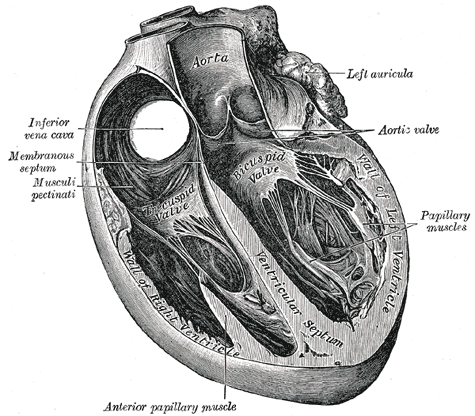
\includegraphics[width=0.7\textwidth]{figures/sample/Gray498.png} 
\caption[Four-chamber illustration of the human heart.]{Four-chamber illustration of the human heart.  Clockwise from upper-left: right atrium, left atrium, left ventricle, right ventricle.}
\label{fig:fourchamber}\end{figure}

The use of acoustic waves for medical diagnosis, inspired by naval sonar, was initially developed in the 1940s \cite{gagliardi_ultrasonography_1996}.  By 1954, the first clinically useful cardiac ultrasound -- examining motion of the mitral valve in stenosis -- was reported \cite{edler_ultrasonic_1957}.  These early scans were one-dimensional images (`A-mode'), sometimes repeated to generate a time axis (`M-mode').   The sector-scanning probe was developed in the 1970s \cite{bom_ultrasonic_1971,griffith_sector_1974}, leading to the `B-mode' that a modern cardiologist would recognise as an echocardiogram.



%% APPENDICES %% 
% Starts lettered appendices, adds a heading in table of contents, and adds a
%    page that just says "Appendices" to signal the end of your main text.
% \startappendices
% Add or remove any appendices you'd like here:
% \begin{savequote}[8cm]
\textlatin{Cor animalium, fundamentum e\longs t vitæ, princeps omnium, Microco\longs mi Sol, a quo omnis vegetatio dependet, vigor omnis \& robur emanat.}

The heart of animals is the foundation of their life, the sovereign of everything within them, the sun of their microcosm, that upon which all growth depends, from which all power proceeds.
  \qauthor{--- William Harvey \cite{harvey_exercitatio_1628}}
\end{savequote}

\chapter{\label{app:1-cardiophys}Review of Cardiac Physiology and Electrophysiology}

\minitoc

Appendices are just like chapters.  Their sections and subsections get numbered and included in the table of contents; figures and equations and tables added up, etc.  Lorem ipsum dolor sit amet, consectetur adipiscing elit. Sed et dui sem. Aliquam dictum et ante ut semper. Donec sollicitudin sed quam at aliquet. Sed maximus diam elementum justo auctor, eget volutpat elit eleifend. Curabitur hendrerit ligula in erat feugiat, at rutrum risus suscipit. Pellentesque habitant morbi tristique senectus et netus et malesuada fames ac turpis egestas. Integer risus nulla, facilisis eget lacinia a, pretium mattis metus. Vestibulum aliquam varius ligula nec consectetur. Maecenas ac ipsum odio. Cras ac elit consequat, eleifend ipsum sodales, euismod nunc. Nam vitae tempor enim, sit amet eleifend nisi. Etiam at erat vel neque consequat.

\section{Anatomy}
\label{sec:anatomy}

Lorem ipsum dolor sit amet, consectetur adipiscing elit. Donec accumsan cursus neque. Pellentesque eget tempor turpis, quis malesuada dui. Proin egestas, sapien sit amet feugiat vulputate, nunc nibh mollis nunc, nec auctor turpis purus sed metus. Aenean consequat leo congue volutpat euismod. Vestibulum et vulputate nisl, at ultrices ligula. Cras pulvinar lacinia ipsum at bibendum. In ac augue ut ante mollis molestie in a arcu.

Etiam vitae quam sollicitudin, luctus tortor eu, efficitur nunc. Vestibulum maximus, ante quis consequat sagittis, augue velit luctus odio, in scelerisque arcu magna id diam. Proin et mauris congue magna auctor pretium id sit amet felis. Maecenas sit amet lorem ipsum. Proin a risus diam. Integer tempus eget est condimentum faucibus. Suspendisse sem metus, consequat vel ante eget, porttitor maximus dui. Nunc dapibus tincidunt enim, non aliquam diam vehicula sed. Proin vel felis ut quam porta tempor. Vestibulum elit mi, dictum eget augue non, volutpat imperdiet eros. Praesent ac egestas neque, et vehicula felis.

Pellentesque malesuada volutpat justo, id eleifend leo pharetra at. Pellentesque feugiat rutrum lobortis. Curabitur hendrerit erat porta massa tincidunt rutrum. Donec tincidunt facilisis luctus. Aliquam dapibus sodales consectetur. Suspendisse lacinia, ipsum sit amet elementum fermentum, nulla urna mattis erat, eu porta metus ipsum vel purus. Fusce eget sem nisl. Pellentesque dapibus, urna vitae tristique aliquam, purus leo gravida nunc, id faucibus ipsum magna aliquet ligula. Lorem ipsum dolor sit amet, consectetur adipiscing elit. Proin sem lacus, rutrum eget efficitur sed, aliquam vel augue. Aliquam ut eros vitae sem cursus ultrices ut ornare urna. Nullam tempor porta enim, in pellentesque arcu commodo quis. Interdum et malesuada fames ac ante ipsum primis in faucibus. Curabitur maximus orci purus, ut molestie turpis pellentesque ut.

Donec lacinia tristique ultricies. Proin dignissim risus ut dolor pulvinar mollis. Proin ac turpis vitae nibh finibus ullamcorper viverra quis felis. Mauris pellentesque neque diam, id feugiat diam vestibulum vitae. In suscipit dui eu libero ultrices, et sagittis nunc blandit. Aliquam at aliquet ex. Nullam molestie pulvinar ex vitae interdum. Praesent purus nunc, gravida id est consectetur, convallis elementum nulla. Praesent ex dolor, maximus eu facilisis at, viverra eget nulla. Donec ullamcorper ante nisi. Sed volutpat diam eros. Nullam egestas neque non tortor aliquet, sed pretium velit tincidunt. Aenean condimentum, est ac vestibulum mattis, quam augue congue augue, mattis ultrices nibh libero non ante. Lorem ipsum dolor sit amet, consectetur adipiscing elit.

Aenean volutpat eros tortor, non convallis sapien blandit et. Maecenas faucibus nulla a magna posuere commodo. Nullam laoreet ante a turpis laoreet malesuada. Phasellus in varius sem. Vestibulum sagittis nibh sed tincidunt blandit. Donec aliquam accumsan odio sit amet lacinia. Integer in tellus diam. Vivamus varius massa leo, vitae ullamcorper metus pulvinar sed. Maecenas nec lorem ornare, elementum est quis, gravida massa. Suspendisse volutpat odio ex, ac ultrices leo ultrices vel. Sed sed convallis ipsum. Pellentesque euismod a nulla sed rhoncus. Sed vehicula urna vitae mi aliquet, non sodales lacus ullamcorper. Duis mattis justo turpis, id tempus est tempus eu. Curabitur vitae hendrerit ligula.

Curabitur non pretium enim, in commodo ligula. Etiam commodo eget ligula a lacinia. Vestibulum laoreet ante tellus, vel congue sapien ornare in. Donec venenatis cursus velit vitae pulvinar. Pellentesque habitant morbi tristique senectus et netus et malesuada fames ac turpis egestas. Suspendisse in metus lectus. Pellentesque gravida dolor eget finibus imperdiet. Duis id molestie tortor. Mauris laoreet faucibus facilisis. Aliquam vitae dictum massa, sit amet dignissim lacus.

Fusce eleifend tellus id ex consequat maximus. Donec ultrices ex ut turpis ornare, non molestie mi placerat. Nulla sit amet auctor nunc, sit amet euismod elit. Phasellus risus tellus, condimentum a metus et, venenatis tristique urna. Cras mattis felis eget ipsum fermentum egestas. Ut augue odio, venenatis id convallis vel, congue quis augue. Maecenas sed maximus est, posuere aliquet tortor. Ut condimentum egestas nisi eu porttitor. Ut mi turpis, posuere id lorem vel, elementum tempor arcu.

Morbi nisl arcu, venenatis non metus ac, ullamcorper scelerisque justo. Nulla et accumsan lorem. Mauris aliquet dui sit amet libero aliquet, in ornare metus porttitor. Integer ultricies urna eu consequat ultrices. Maecenas a justo id purus ultricies posuere sed et quam. Cum sociis natoque penatibus et magnis dis parturient montes, nascetur ridiculus mus. Sed eleifend risus quis aliquet gravida. Nullam ac erat porta est bibendum dictum in a dolor. Nam eget turpis viverra, vulputate lectus eget, mattis ligula. Nam at tellus eget dui lobortis sodales et ut augue. In vestibulum diam eget mi cursus, ut tincidunt nulla pellentesque.

Aliquam erat volutpat. Sed ultrices massa id ex mattis bibendum. Nunc augue magna, ornare at aliquet gravida, vehicula sed lorem. Quisque lobortis ipsum eu posuere eleifend. Duis bibendum cursus viverra. Nam venenatis elit leo, vitae feugiat quam aliquet sed. Cras velit est, tempus ac lorem sed, pharetra lobortis ipsum. Donec suscipit gravida interdum. Nunc non finibus est. Nullam turpis elit, tempus non ante.

\section{Mechanical Cycle}

Lorem ipsum dolor sit amet, consectetur adipiscing elit. Aenean tellus est, suscipit sed facilisis quis, malesuada at ipsum. Nam tristique urna quis quam iaculis, et mattis orci pretium. Praesent euismod elit vel metus commodo ultrices. Vestibulum et tincidunt ex, in molestie ex. Donec ullamcorper sollicitudin accumsan. Etiam ac leo turpis. Duis a tortor felis. Nullam sollicitudin eu purus ac hendrerit. Nam hendrerit ligula libero, eget finibus orci bibendum a. Aenean ut ipsum magna.

Ut viverra, sapien sed accumsan blandit, nisi sem tempus tellus, at suscipit magna erat ornare nunc. Proin lacinia, nisi ut rutrum malesuada, nibh quam pellentesque nunc, sit amet consectetur purus felis ac tortor. Suspendisse lacinia ipsum eu sapien pellentesque mattis. Mauris ipsum nunc, placerat non diam vel, efficitur laoreet nunc. Sed lobortis, ipsum eget gravida facilisis, sem nulla viverra mi, in placerat eros sem viverra lacus. Aliquam porta aliquet diam vel commodo. Nulla facilisi. Duis erat libero, lobortis vel hendrerit vitae, sagittis id dui. Nulla pretium eros nec quam tincidunt, vel luctus mi aliquam. Integer imperdiet purus in est tristique venenatis. Ut pellentesque, nunc vitae iaculis ultricies, urna turpis dignissim risus, a laoreet felis magna nec erat.

Quisque sollicitudin faucibus ligula, et egestas nibh dictum sit amet. Proin eu mi a lectus congue pretium eu quis arcu. Suspendisse vehicula libero eu ipsum aliquam, vel elementum nibh mattis. Sed sed sapien vitae turpis tristique pulvinar a ut metus. Etiam semper gravida est, mollis gravida est porta ac. Proin eget tincidunt erat. Maecenas ultrices erat eget purus ultricies, ut lacinia arcu dictum. Nam et nisi sit amet ex congue mattis vel eget lorem. Aliquam erat volutpat. Pellentesque porttitor nibh vitae elementum consectetur. Aenean et est lobortis, congue sapien non, ullamcorper sapien. Ut facilisis sem non dapibus vehicula.

Mauris euismod odio dolor, sit amet gravida mauris placerat et. Curabitur nec dolor non nibh molestie lobortis dignissim non ante. Nullam rutrum lobortis ultrices. Aenean ex erat, elementum sed maximus id, posuere id quam. Proin rutrum ex elit, pretium aliquam risus finibus at. Aenean egestas orci velit, sed aliquet sapien condimentum a. Duis consequat, arcu eu viverra venenatis, dolor lorem gravida lectus, non aliquet nisi sem at augue. Donec laoreet blandit luctus. Aenean vehicula nisl vel faucibus luctus. Sed ut semper velit, vitae laoreet magna. Sed at interdum magna.

Sed iaculis faucibus odio, eu aliquam purus efficitur vel. Cras at nulla ac enim congue varius ut et nulla. Integer blandit mattis augue.

\section{Electrical Cycle}
\label{sec:electcycle}

Lorem ipsum dolor sit amet, consectetur adipiscing elit. In faucibus condimentum rhoncus. Ut dictum nisl id risus gravida lobortis. Sed vehicula mollis tellus ut varius. Fusce eget egestas dui, et commodo dui. Proin sollicitudin interdum tempus. Nullam in elit a enim fringilla bibendum. Vestibulum sodales pellentesque condimentum. Nulla facilisi. Nunc et dolor in nulla eleifend dictum at vel ligula. Aliquam ut velit non elit ullamcorper porta ac et ex. Fusce ornare magna non nunc vestibulum, eget molestie quam dictum. In interdum aliquam odio, in posuere tellus convallis quis. Curabitur non diam elit. Proin vulputate orci diam, a tincidunt ante luctus eu. Ut a viverra ligula. Curabitur pulvinar tempus tellus eget suscipit.

Aliquam posuere massa at ante dapibus congue. Curabitur ullamcorper tortor eget consectetur aliquet. Mauris tempor magna id mauris fringilla, a varius erat blandit. Nam eleifend ullamcorper placerat. Phasellus augue tortor, volutpat bibendum lorem nec, fringilla volutpat nisl. Mauris cursus urna metus, vel eleifend orci iaculis ut. Sed sit amet scelerisque massa, quis consequat dui. Donec semper sem dui, ac placerat velit egestas vel. Nulla facilisi. Quisque tellus eros, sagittis malesuada augue ut, faucibus dictum nulla. Vestibulum non dapibus erat, ut consequat libero. Ut turpis mi, dapibus commodo libero lobortis, maximus vestibulum lectus. Vestibulum sit amet sapien dapibus, tincidunt leo in, suscipit arcu. Sed in erat bibendum, laoreet eros eu, pellentesque justo. Nulla sodales purus neque, eget maximus ipsum consequat at. Maecenas a nisl sagittis, tempus ipsum sed, dictum mauris.

Suspendisse posuere odio lacus, at auctor tortor vehicula sed. Phasellus suscipit ornare enim vitae placerat. Sed viverra purus vel sapien tempor, quis iaculis erat laoreet. Aenean vel nunc vestibulum, ornare nunc ac, mollis urna. Aenean ultrices felis ipsum, ac semper est ullamcorper in. Donec in justo varius, egestas tortor ut, venenatis augue. Duis mattis, ligula quis lacinia fringilla, tellus neque accumsan ipsum, vitae tempor metus elit vel nibh. Curabitur porttitor urna nec sapien tempor, et porttitor velit malesuada.

Suspendisse aliquam nisl quis placerat vulputate. Proin dapibus ipsum ac ante sagittis, volutpat auctor sem dapibus. Nam in facilisis odio. Integer ante mauris, eleifend et pulvinar in, venenatis quis ligula. Phasellus posuere sollicitudin tortor eget euismod. Maecenas mollis tortor eget justo vulputate sagittis. Etiam hendrerit massa quis ex molestie sodales. Quisque facilisis erat lacus, id convallis sem suscipit bibendum. Integer dui urna, pharetra sed porta sed, bibendum ut odio. Donec placerat at lectus egestas consequat. Sed id rhoncus est, vitae vulputate sapien. Fusce tempus quam lorem, id ornare turpis sodales sed. Integer aliquet urna eget condimentum consequat. Vestibulum quis dui vel ligula posuere luctus id nec turpis.

Nam vitae placerat lacus. Mauris scelerisque interdum volutpat. Nunc aliquet tristique enim, sit amet molestie felis ullamcorper vitae. Nullam sollicitudin orci orci, in condimentum tellus consectetur in. Nam id justo justo. Fusce eget finibus est. Proin id tortor nec quam cursus vehicula. Aliquam ultrices eros eros, a tincidunt elit eleifend auctor.

Nullam consectetur dapibus ligula sit amet efficitur. Nunc non posuere sapien. Vivamus dui nisl, aliquam id ipsum non, pulvinar ornare neque. Nunc rhoncus pretium congue. Fusce id laoreet enim. Cras sed massa in eros bibendum auctor in nec sem. Nam commodo, velit id porta consequat, mi arcu gravida lorem, ut aliquam elit ante quis dui. Quisque in massa sed nibh blandit dictum.

Vestibulum molestie consectetur porttitor. Donec tincidunt vel orci at pharetra. Nullam id felis sit amet nulla tempus lacinia. Integer egestas ullamcorper massa, ut ultricies diam congue sit amet. Cras sit amet velit at nibh vehicula finibus a et lorem. Cras odio metus, venenatis ut ultrices non, ornare ac orci. Morbi et nulla dui. Mauris dictum molestie nibh, eu efficitur lorem accumsan quis.

\section{Cellular Electromechanical Coupling}
\label{sec:electromech}

Lorem ipsum dolor sit amet, consectetur adipiscing elit. Nullam vitae consectetur metus, ac maximus ex. Quisque vitae ex eu lectus ultricies consequat vel non lorem. Etiam odio ipsum, tempus ut lobortis in, molestie ac leo. Vivamus mollis feugiat bibendum. Vestibulum eget venenatis quam. Aenean faucibus, massa sed ullamcorper porta, arcu nunc iaculis velit, quis consectetur purus neque placerat nibh. Vestibulum elit nunc, dignissim vulputate venenatis et, sodales non massa. Proin leo ligula, vehicula eu aliquam varius, posuere a dolor. Donec iaculis auctor neque, sit amet gravida libero porta vel. Vivamus consequat elementum lacus, at bibendum mauris egestas nec. Fusce fermentum diam eu dolor ornare, vitae vestibulum leo interdum. Morbi luctus libero quis dictum laoreet. Etiam semper porta ante, vel ullamcorper enim sodales quis.

Nullam eu nisi faucibus, fermentum ex auctor, tempor arcu. Phasellus condimentum erat mi, condimentum malesuada ligula congue venenatis. Nullam gravida imperdiet urna quis cursus. Ut tempus nec purus eget posuere. Cras non nulla sit amet justo aliquet pellentesque nec sed eros. Nam aliquam nisl urna, in placerat magna gravida venenatis. Donec interdum vel magna ullamcorper molestie. Nunc felis neque, rhoncus fringilla faucibus sit amet, ultrices sed magna. Maecenas malesuada hendrerit diam in ultrices. Nam libero urna, volutpat ut auctor eget, interdum sed odio. Vestibulum suscipit mauris nec augue ornare, ut eleifend nulla gravida. Proin imperdiet, mauris quis consectetur porta, leo dui convallis leo, id lobortis massa diam eu libero. Aenean hendrerit vel ante aliquam venenatis. Pellentesque bibendum pretium odio, ut sagittis lectus feugiat a. Donec porttitor vulputate lacus.

Nunc volutpat efficitur lacus in aliquet. Nullam non iaculis diam, at ultrices diam. Proin vehicula vulputate cursus. Morbi tempus sapien id urna lobortis interdum. Maecenas elementum sagittis elementum. Donec at sodales velit, a posuere tortor. Nulla id hendrerit tortor. Sed semper velit in magna sagittis pulvinar. Nulla nec arcu molestie, ultricies sapien sit amet, sollicitudin nisi. Donec nisi massa, suscipit ut dignissim quis, lacinia id leo.

Suspendisse ut mi metus. Morbi tincidunt ligula in porttitor consectetur. Integer eu urna urna. Suspendisse potenti. Mauris sit amet felis eu diam auctor ullamcorper. Morbi in porta nisi. Nam ante tortor, venenatis vitae tempor sed, sagittis vitae velit. In semper orci sit amet nisi ullamcorper varius. Aenean dignissim ultrices imperdiet. Maecenas lacinia enim id neque porttitor iaculis. Curabitur laoreet ante ut urna dignissim, id sollicitudin metus consectetur. Aenean massa ipsum, auctor vel ante vel, blandit dignissim libero. Fusce interdum ac magna et interdum.



%%%%% REFERENCES

% JEM: Quote for the top of references (just like a chapter quote if you're using them).  Comment to skip.
\begin{savequote}[8cm]
The first kind of intellectual and artistic personality belongs to the hedgehogs, the second to the foxes \dots
  \qauthor{--- Sir Isaiah Berlin \cite{berlin_hedgehog_2013}}
\end{savequote}

\setlength{\baselineskip}{0pt} % JEM: Single-space References

{\renewcommand*\MakeUppercase[1]{#1}%
\printbibliography[heading=bibintoc,title={\bibtitle}]}


\end{document}
